\documentclass[8pt]{beamer}
\usepackage{../../shared/styles/custom}
\usepackage{../../shared/styles/conventions}
\usepackage{tikz}
\usetikzlibrary{positioning,shapes,arrows}

% Remove navigation symbols
\setbeamertemplate{navigation symbols}{}

% Add fitpic for image fitting
\newcommand{\fitpic}[1]{\begin{adjustbox}{max width=\linewidth, max totalheight=0.78\textheight}#1\end{adjustbox}}

%\beamerdefaultoverlayspecification{<+->}
% \newcommand{\data}{\mathcal{D}}
% \newcommand\Item[1][]{%
%   \ifx\relax#1\relax  \item \else \item[#1] \fi
%   \abovedisplayskip=0pt\abovedisplayshortskip=0pt~\vspace*{-\baselineskip}}

\newcommand*{\Comb}[2]{{}^{#1}C_{#2}}%

\graphicspath{ {../assets/ensemble/figures/} }




\title{Ensemble Learning}
\date{\today}
\author{Nipun Batra and teaching staff}
\institute{IIT Gandhinagar}
\begin{document}
\maketitle

\begin{frame}{Table of Contents}
\tableofcontents
\end{frame}

\section{Introduction to Ensemble Learning}

\begin{frame}{What is Ensemble Learning?}
\begin{alertbox}{The Core Idea}
\textbf{``The wisdom of crowds''}: Combine multiple models to make better predictions than any single model could achieve alone.
\end{alertbox}

\begin{keypointsbox}
\textbf{Key Insight:}
\begin{itemize}
\item Individual models make different mistakes
\item By combining them intelligently, we can reduce overall error
\item Most Kaggle competition winners use ensemble methods!
\end{itemize}
\end{keypointsbox}
\end{frame}

\begin{frame}{Real-World Analogy: Medical Diagnosis}
\begin{examplebox}{Why Do We Seek Second Opinions?}
\textbf{Single Doctor:}
\begin{itemize}
\item Might miss subtle symptoms
\item Could have personal biases
\item Limited by individual experience
\end{itemize}

\textbf{Multiple Doctors (Ensemble):}
\begin{itemize}
\item Different perspectives and expertise
\item Collective wisdom reduces misdiagnosis
\item More robust and reliable decisions
\end{itemize}
\end{examplebox}
\end{frame}

\begin{frame}{Simple Ensemble Examples}
\begin{columns}
\begin{column}{0.5\textwidth}
\begin{examplebox}{Classification}
\textbf{Problem:} Spam detection

\textbf{Individual Predictions:}
\begin{itemize}
\item Model 1: Spam 
\item Model 2: Spam 
\item Model 3: Not Spam 
\end{itemize}

\textbf{Ensemble (Majority Vote):} Spam 
\end{examplebox}
\end{column}

\begin{column}{0.5\textwidth}
\begin{examplebox}{Regression}
\textbf{Problem:} House price prediction

\textbf{Individual Predictions:}
\begin{itemize}
\item Model 1: \$420K
\item Model 2: \$450K
\item Model 3: \$430K
\end{itemize}

\textbf{Ensemble (Average):} \$433K
\end{examplebox}
\end{column}
\end{columns}
\end{frame}


\begin{frame}{Why Do Ensembles Work? Three Key Reasons}
\begin{alertbox}{Based on Ensemble Methods in ML by Dietterich}
\textbf{Three fundamental reasons why combining models works better:}
\end{alertbox}

\begin{keypointsbox}
\begin{enumerate}
\item \textbf{Statistical}: Limited data → Multiple valid hypotheses
\item \textbf{Computational}: Models get stuck in local optima
\item \textbf{Representational}: Individual models have limitations
\end{enumerate}
\end{keypointsbox}
\end{frame}

\begin{frame}{Reason 1: Statistical Problem}
\begin{definitionbox}{The Statistical Challenge}
When data is limited, many competing hypotheses can achieve the same accuracy on training data.
\end{definitionbox}

\begin{examplebox}{Decision Trees Example}
\begin{itemize}
\item Same dataset → multiple valid trees
\item Combining reduces risk of picking the ``wrong'' one
\end{itemize}
\end{examplebox}

\begin{center}
\fitpic{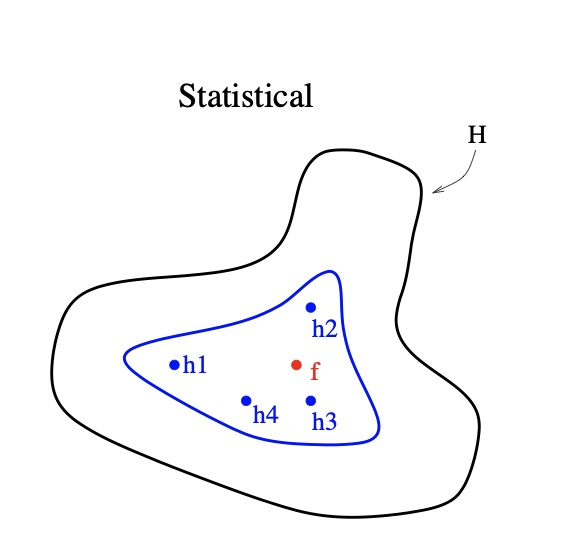
\includegraphics[scale=0.2]{../assets/ensemble/diagrams/statistical.jpg}}
\end{center}
\end{frame}

\begin{frame}{Reason 2: Computational Problem}
\begin{definitionbox}{The Computational Challenge}
Learning algorithms can get stuck in local optima or use greedy strategies.
\end{definitionbox}

\begin{examplebox}{Examples}
\begin{itemize}
\item Decision trees: greedy splits
\item Neural networks: local minima
\item Different runs → different solutions
\end{itemize}
\end{examplebox}

\begin{center}
\fitpic{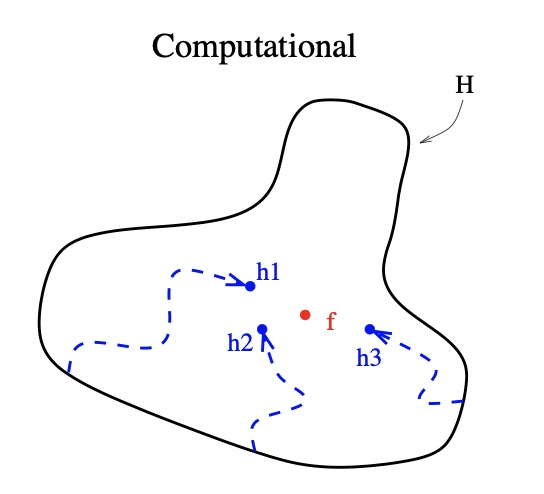
\includegraphics[scale=0.2]{../assets/ensemble/diagrams/computational.jpg}}
\end{center}
\end{frame}

\begin{frame}{Reason 3: Representational Problem}
\begin{definitionbox}{The Representational Challenge}
Some models cannot learn the true form of the target function.
\end{definitionbox}

\begin{examplebox}{Limitations}
\begin{itemize}
\item Decision trees: axis-parallel splits only
\item Linear models: no non-linear relationships
\item Each model has inherent biases
\end{itemize}
\end{examplebox}

\begin{center}
\fitpic{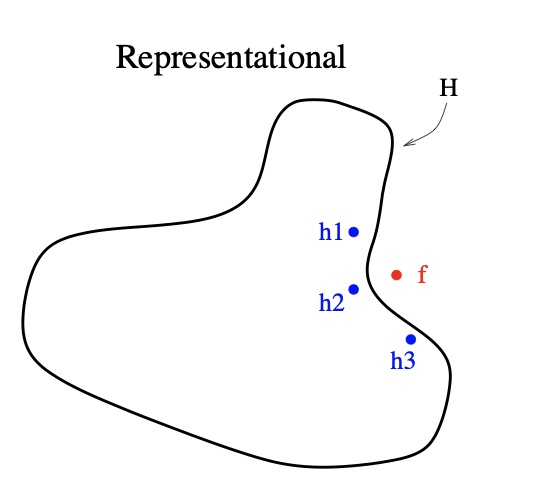
\includegraphics[scale=0.2]{../assets/ensemble/diagrams/representational.jpg}}
\end{center}
\end{frame}

\begin{frame}{Visual Example: Decision Trees vs Random Forest}
\begin{alertbox}{Representation Comparison}
\textbf{Question:} How do individual decision trees compare to their ensemble?
\end{alertbox}

\begin{figure}[htp]
  \centering
  \begin{notebookbox}{https://nipunbatra.github.io/ml-teaching/notebooks/ensemble-representation.html}
    \fitpic{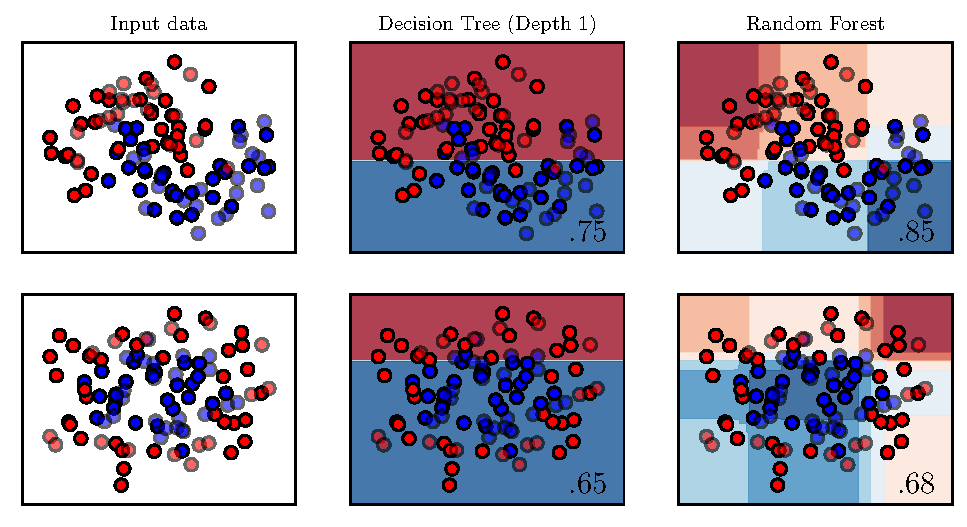
\includegraphics[scale=0.6]{../assets/ensemble/figures/1-representation.pdf}}
  \end{notebookbox}
\end{figure}

\begin{keypointsbox}
\textbf{Observation:} Individual trees create rigid, rectangular decision boundaries
\end{keypointsbox}
\end{frame}

\begin{frame}{Random Forest: The Power of Combination}
\begin{examplebox}{Ensemble Effect}
\textbf{Result:} Combining multiple trees creates smoother, more flexible decision boundaries
\end{examplebox}

  \begin{figure}[htp]
    \centering
    \begin{notebookbox}{https://nipunbatra.github.io/ml-teaching/notebooks/ensemble-representation.html}
      \fitpic{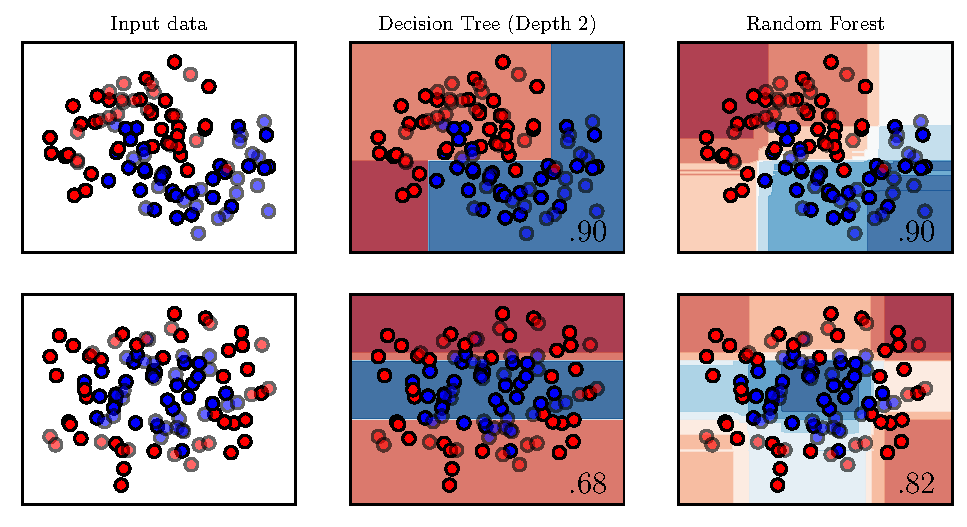
\includegraphics[scale=0.6]{../assets/ensemble/figures/2-representation.pdf}}
    \end{notebookbox}
  \end{figure}
  
\begin{keypointsbox}
\textbf{Key Insight:} The ensemble overcomes individual model limitations!
\end{keypointsbox}
  \end{frame}




\begin{frame}{When Do Ensembles Work? Two Key Requirements}
\begin{definitionbox}{Necessary and Sufficient Conditions}
For an ensemble to outperform individual members, models must be:
\begin{enumerate}
\item \textbf{Accurate}: Better than random guessing
\item \textbf{Diverse}: Make different errors on new data
\end{enumerate}
\end{definitionbox}

\begin{keypointsbox}
\textbf{Key Terms:}
\begin{itemize}
\item \textbf{Accurate}: Error rate < 50\% (better than coin flip)
\item \textbf{Diverse}: Models disagree on different examples
\end{itemize}
\end{keypointsbox}
\end{frame}

\begin{frame}{Diversity: The Magic Ingredient}
\begin{columns}
\begin{column}{0.5\textwidth}
\begin{alertbox}{Identical Models (No Diversity)}
\textbf{Scenario:} All three models make the same mistakes

When $h_1(x)$ is wrong:
\begin{itemize}
\item $h_2(x)$ is also wrong
\item $h_3(x)$ is also wrong
\item Ensemble prediction: \textcolor{red}{Wrong}
\end{itemize}
\end{alertbox}
\end{column}

\begin{column}{0.5\textwidth}
\begin{examplebox}{Diverse Models}
\textbf{Scenario:} Models make different mistakes

When $h_1(x)$ is wrong:
\begin{itemize}
\item $h_2(x)$ might be correct
\item $h_3(x)$ might be correct
\item Ensemble prediction: \textcolor{green}{Correct!}
\end{itemize}
\end{examplebox}
\end{column}
\end{columns}

\begin{keypointsbox}
\textbf{Bottom Line:} Diversity allows the ensemble to correct individual model errors!
\end{keypointsbox}
\end{frame}
\begin{frame}{Mathematical Proof: Why Ensembles Work}
\begin{definitionbox}{Majority Voting Analysis}
\textbf{Setup:} 3 models, each with error probability $\varepsilon = 0.3$

\textbf{Ensemble fails when:} 2 or 3 models are wrong
\end{definitionbox}

\begin{examplebox}{Calculation}
$P(\text{ensemble wrong}) = \binom{3}{2}\varepsilon^2(1-\varepsilon) + \binom{3}{3}\varepsilon^3$

$= 3 \times 0.3^2 \times 0.7 + 1 \times 0.3^3$

$= 0.189 + 0.027 = \mathbf{0.216}$
\end{examplebox}

\begin{keypointsbox}
\textbf{Result:} Ensemble error (21.6\%) < Individual error (30\%)!
\end{keypointsbox}
\end{frame}

\begin{frame}{The Power of Scaling: More Models = Better Performance}
\begin{columns}
\begin{column}{0.5\textwidth}
\begin{examplebox}{Good Individual Models ($\varepsilon = 0.3$)}
\begin{center}
\begin{tabular}{c|c}
\# Models & Ensemble Error \\
\hline
1 & 30.0\% \\
3 & 21.6\% \\
5 & 16.3\% \\
\end{tabular}
\end{center}

\textcolor{green}{\textbf{Ensembles help!}}
\end{examplebox}
\end{column}

\begin{column}{0.5\textwidth}
\begin{alertbox}{Poor Individual Models ($\varepsilon = 0.6$)}
\begin{center}
\begin{tabular}{c|c}
\# Models & Ensemble Error \\
\hline
1 & 60.0\% \\
3 & 64.8\% \\
5 & 68.3\% \\
\end{tabular}
\end{center}

\textcolor{red}{\textbf{Ensembles hurt!}}
\end{alertbox}
\end{column}
\end{columns}

\begin{keypointsbox}
\textbf{Key Insight:} Ensembles only help when base models are better than random!
\end{keypointsbox}
\end{frame}

\begin{frame}{When Ensembles Fail: Common Pitfalls}
\begin{alertbox}{Ensemble Limitations}
\textbf{Ensembles DON'T work well when:}
\end{alertbox}

\begin{columns}
\begin{column}{0.5\textwidth}
\begin{examplebox}{Poor Base Models}
\begin{itemize}
\item Individual accuracy < 50\%
\item Models worse than random guessing
\item Garbage in → Garbage out
\end{itemize}
\end{examplebox}
\end{column}

\begin{column}{0.5\textwidth}
\begin{examplebox}{Lack of Diversity}
\begin{itemize}
\item All models make same mistakes
\item High correlation between predictions
\item No complementary strengths
\end{itemize}
\end{examplebox}
\end{column}
\end{columns}

\begin{keypointsbox}
\textbf{Solution:} Ensure base models are accurate AND diverse!
\end{keypointsbox}
\end{frame}

\section{Bagging: Bootstrap Aggregation}

\begin{frame}{What is Bagging?}
\begin{definitionbox}{Bagging = Bootstrap + Aggregation}
\textbf{Goal:} Create diverse models from a single dataset to reduce variance
\end{definitionbox}

\begin{keypointsbox}
\textbf{Key Insight:} Even with the same algorithm and same data, we can create different models by training on different subsets!
\end{keypointsbox}

\begin{alertbox}{The Challenge}
\textbf{Problem:} How do we get different training sets from one dataset?

\textbf{Solution:} Bootstrap sampling (sampling with replacement)
\end{alertbox}
\end{frame}

\begin{frame}{Bootstrap Sampling: The Core Technique}
\begin{examplebox}{Bootstrap Process}
\textbf{Original Dataset:} $D = \{D_1, D_2, D_3, \ldots, D_n\}$

\textbf{For each model:} Create new dataset by sampling $n$ examples \emph{with replacement}
\end{examplebox}

\begin{columns}
\begin{column}{0.5\textwidth}
\begin{definitionbox}{Bootstrap Sample 1}
$D_1, D_3, D_6, D_1, D_5, \ldots$

\textcolor{blue}{Notice: $D_1$ appears twice!}
\end{definitionbox}
\end{column}

\begin{column}{0.5\textwidth}
\begin{definitionbox}{Bootstrap Sample 2}
$D_2, D_4, D_1, D_n, D_3, \ldots$

\textcolor{blue}{Different sample, different model!}
\end{definitionbox}
\end{column}
\end{columns}

\begin{keypointsbox}
\textbf{Result:} Each bootstrap sample is slightly different → Diverse models!
\end{keypointsbox}
\end{frame}

\begin{frame}{Bagging Example: The Dataset}
\begin{alertbox}{Classification Problem}
\textbf{Task:} Classify points as red or blue circles

\textbf{Challenge:} Points (3,3) and (5,8) are outliers/anomalies
\end{alertbox}

  \begin{center}
  \fitpic{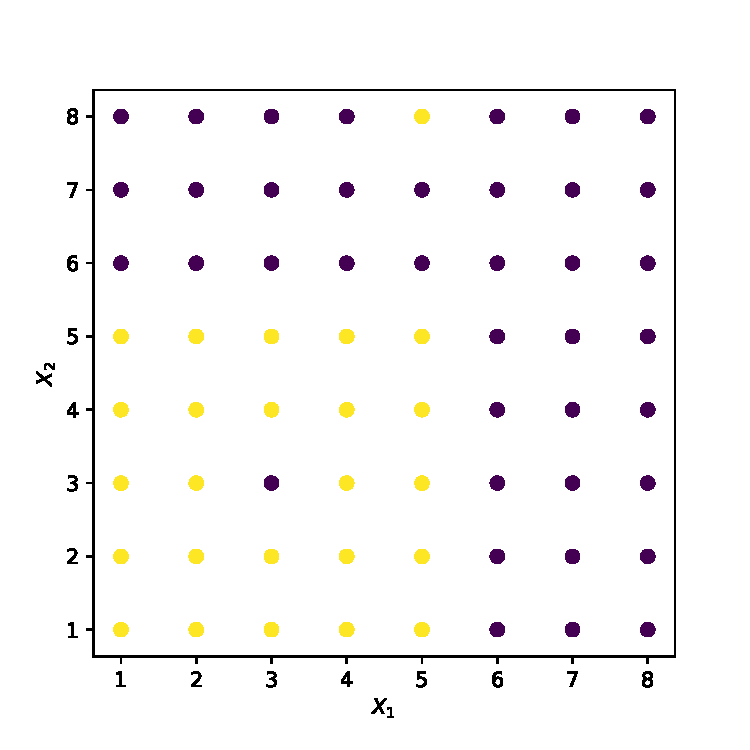
\includegraphics[width = 0.6\textwidth]{../assets/ensemble/figures/dataset}}
  \end{center}

\begin{keypointsbox}
\textbf{Question:} How will a single decision tree handle these outliers?
\end{keypointsbox}
\end{frame}

\begin{frame}{Single Decision Tree: Overfitting Problem}
\begin{examplebox}{Deep Decision Tree (Depth = 6)}
\textbf{Result:} Complex boundary that memorizes outliers
\end{examplebox}

  \begin{center}
  \fitpic{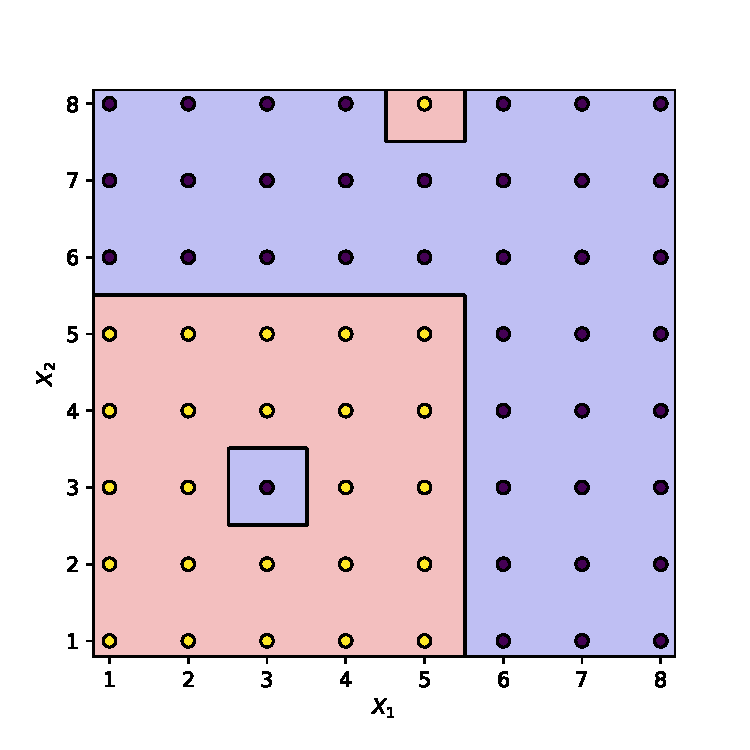
\includegraphics[width = 0.6\textwidth]{../assets/ensemble/figures/strong-tree}}
  \end{center}

\begin{alertbox}{The Problem}
\textbf{High Variance:} Small changes in data → Very different decision boundaries
\end{alertbox}
\end{frame}

\begin{frame}{Bootstrap Samples: Part 1}
\begin{examplebox}{Creating Diverse Training Sets}
Generate different bootstrap samples from original dataset
\end{examplebox}

\begin{center}
\begin{columns}
\begin{column}{0.45\textwidth}
\centering
\textbf{Sample 1}

\fitpic{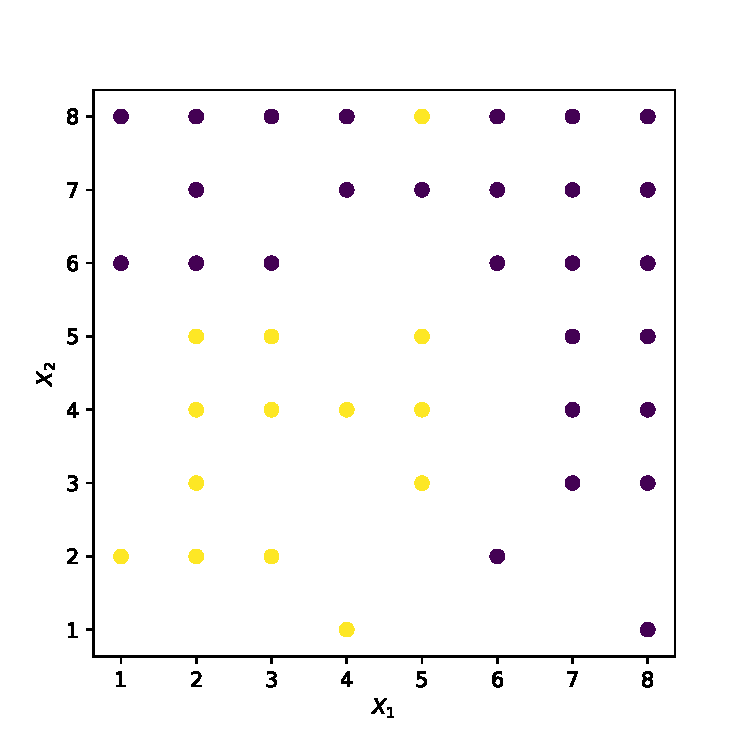
\includegraphics[width = 0.9\textwidth]{../assets/ensemble/figures/dataset-rnd-0}}
\end{column}

\begin{column}{0.45\textwidth}
\centering
\textbf{Sample 2}

\fitpic{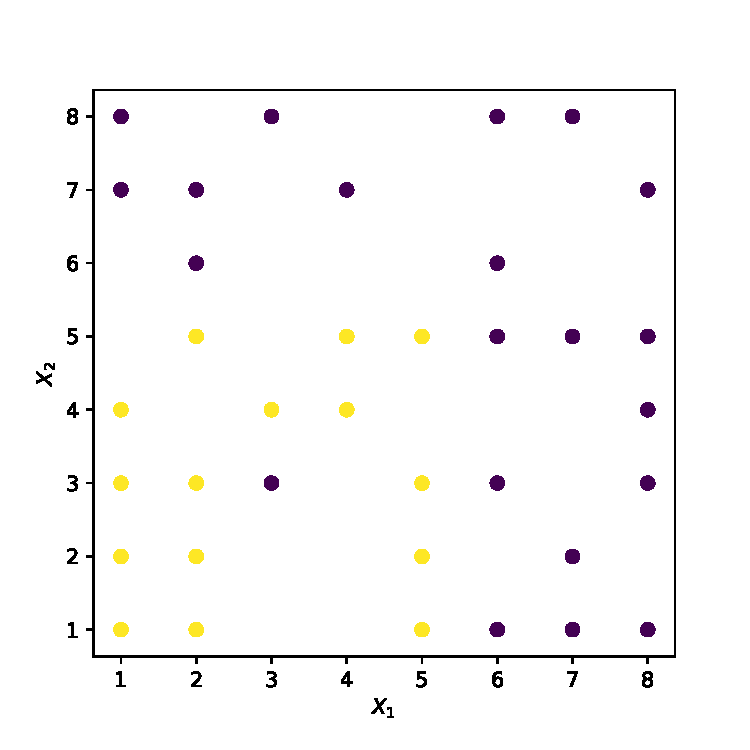
\includegraphics[width = 0.9\textwidth]{../assets/ensemble/figures/dataset-rnd-1}}
\end{column}
\end{columns}
\end{center}
\end{frame}

\begin{frame}{Bootstrap Samples: Part 2}
\begin{center}
\begin{columns}
\begin{column}{0.45\textwidth}
\centering
\textbf{Sample 3}

\fitpic{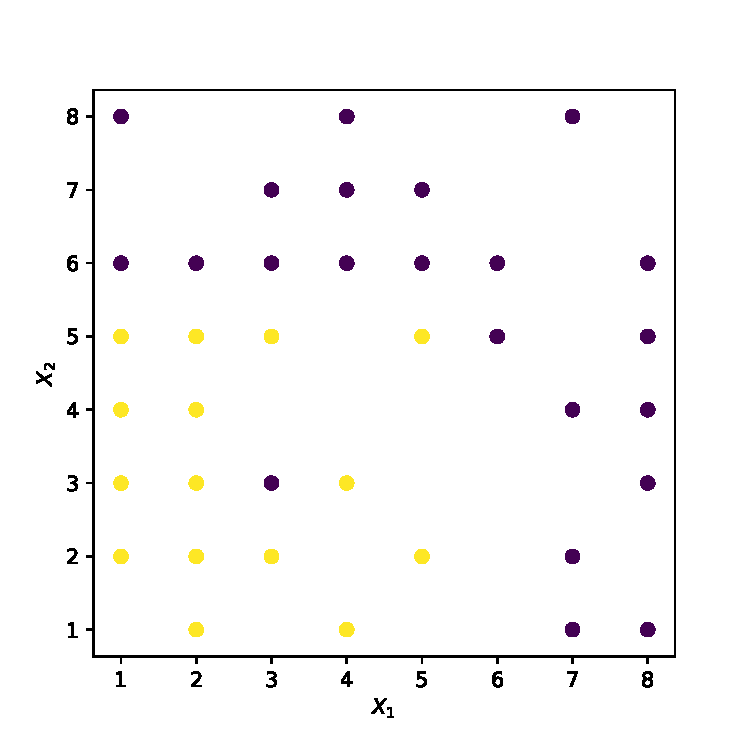
\includegraphics[width = 0.9\textwidth]{../assets/ensemble/figures/dataset-rnd-2}}
\end{column}

\begin{column}{0.45\textwidth}
\centering
\textbf{Sample 4}

\fitpic{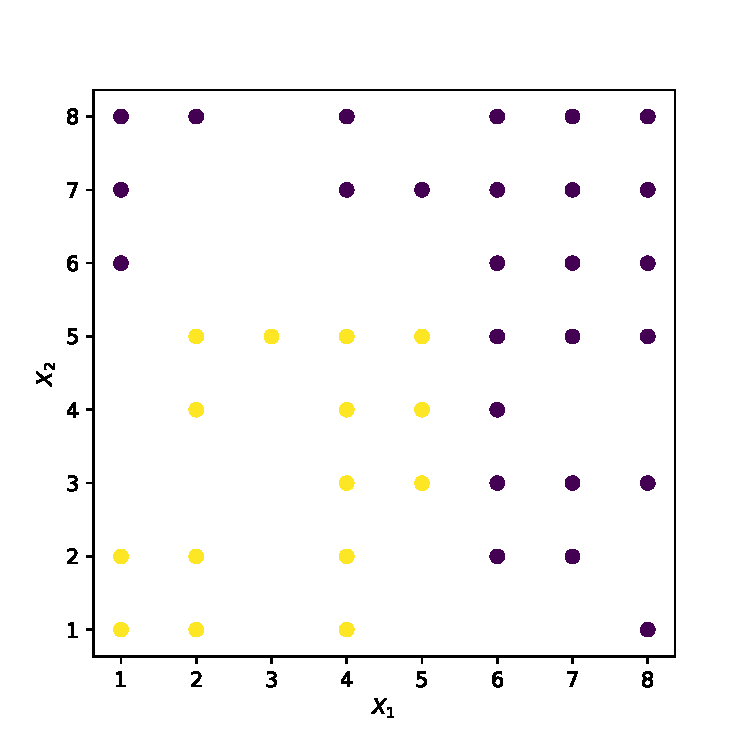
\includegraphics[width = 0.9\textwidth]{../assets/ensemble/figures/dataset-rnd-3}}
\end{column}
\end{columns}
\end{center}

\begin{keypointsbox}
\textbf{Key Insight:} Each sample has different combinations of points!
\end{keypointsbox}
\end{frame}


\begin{frame}{Bagging : Classification Example}
  \vspace{0.3cm}
  \begin{columns}
    \pause  \begin{column}{0.3\textwidth}
      \centering
      Round - 1\\

      \fitpic{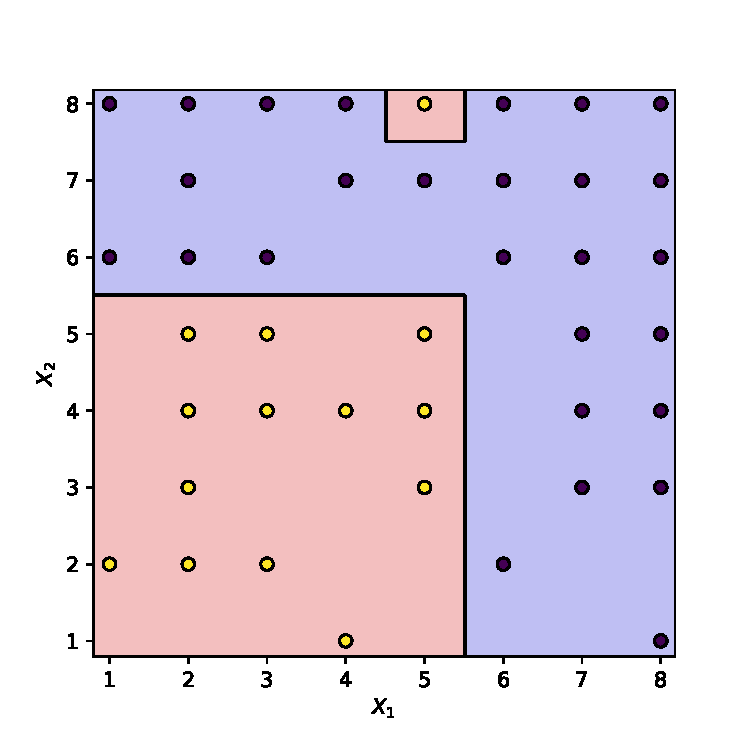
\includegraphics[width = 0.9\textwidth]{../assets/ensemble/figures/decision-boundary-0}}
      Tree Depth = 4

    \end{column}
    \pause  \begin{column}{0.3\textwidth}
      \centering
      Round - 2\\

      \fitpic{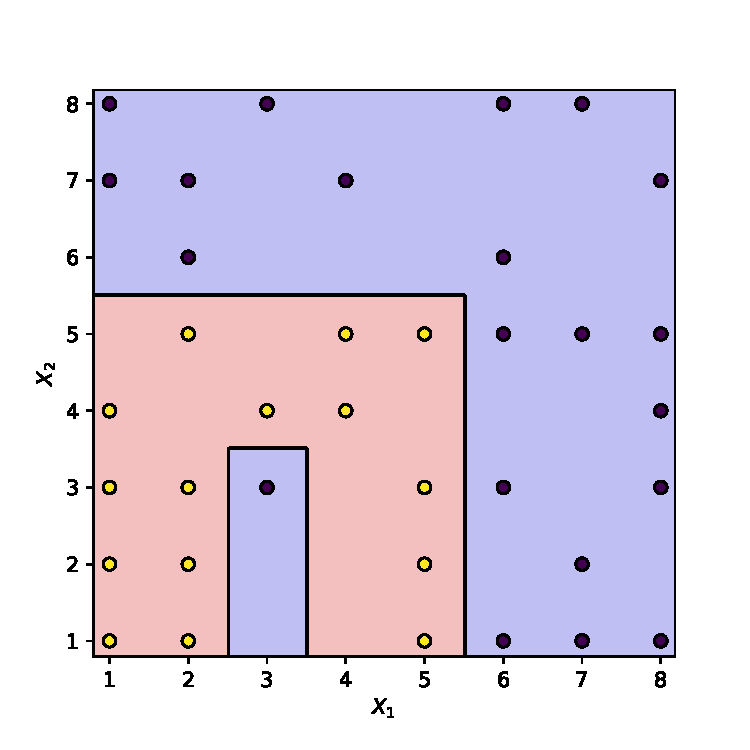
\includegraphics[width = 0.9\textwidth]{../assets/ensemble/figures/decision-boundary-1}}
      Tree Depth = 5

    \end{column}
    \pause  \begin{column}{0.3\textwidth}
      \centering
      Round - 3\\

      \fitpic{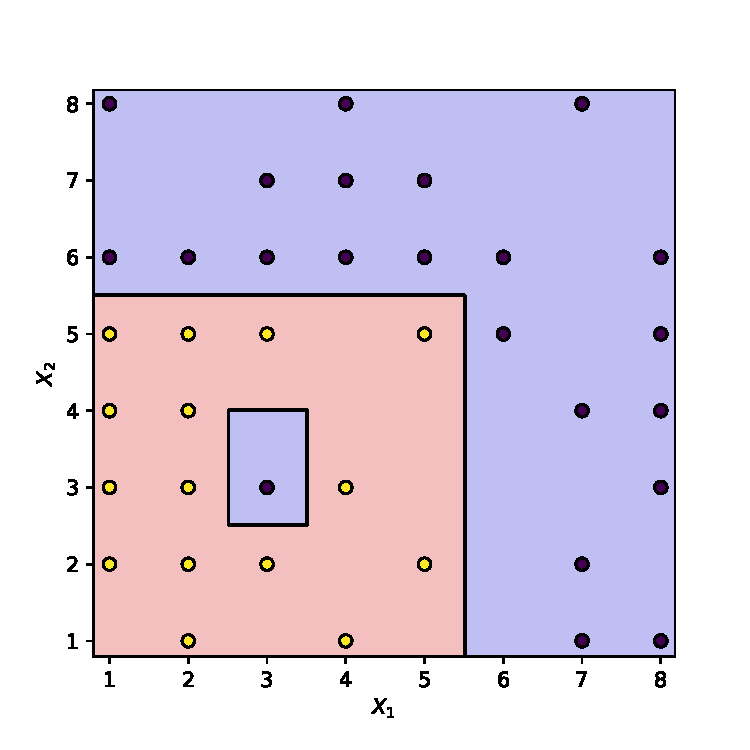
\includegraphics[width = 0.9\textwidth]{../assets/ensemble/figures/decision-boundary-2}}
      Tree Depth = 5

    \end{column}

  \end{columns}
  \vspace{0.5cm}
  \pause  \begin{columns}
    \begin{column}{0.3\textwidth}
      \centering
      Round - 4\\

      \fitpic{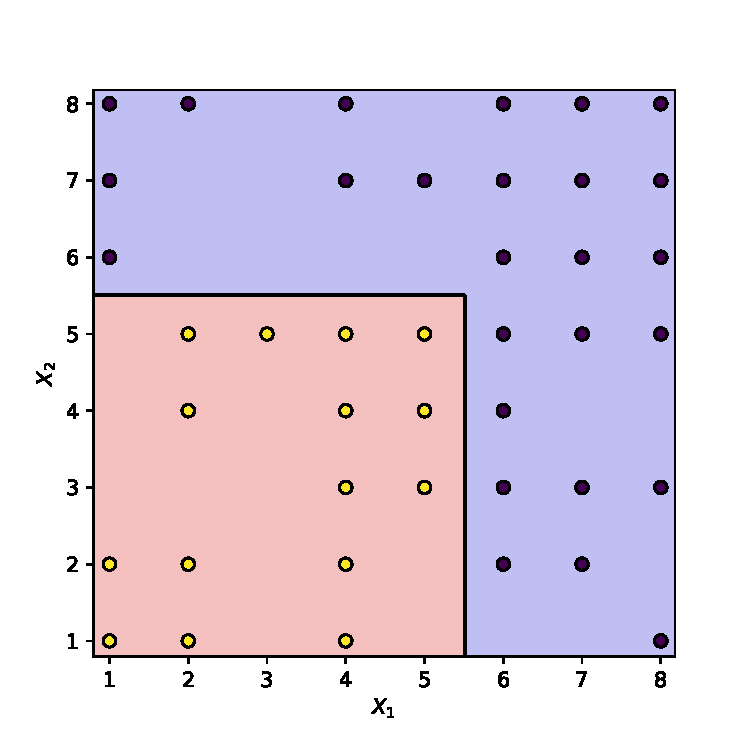
\includegraphics[width = 0.9\textwidth]{../assets/ensemble/figures/decision-boundary-3}}
      Tree Depth = 2

    \end{column}
    \pause  \begin{column}{0.3\textwidth}
      \centering
      Round - 5\\

      \fitpic{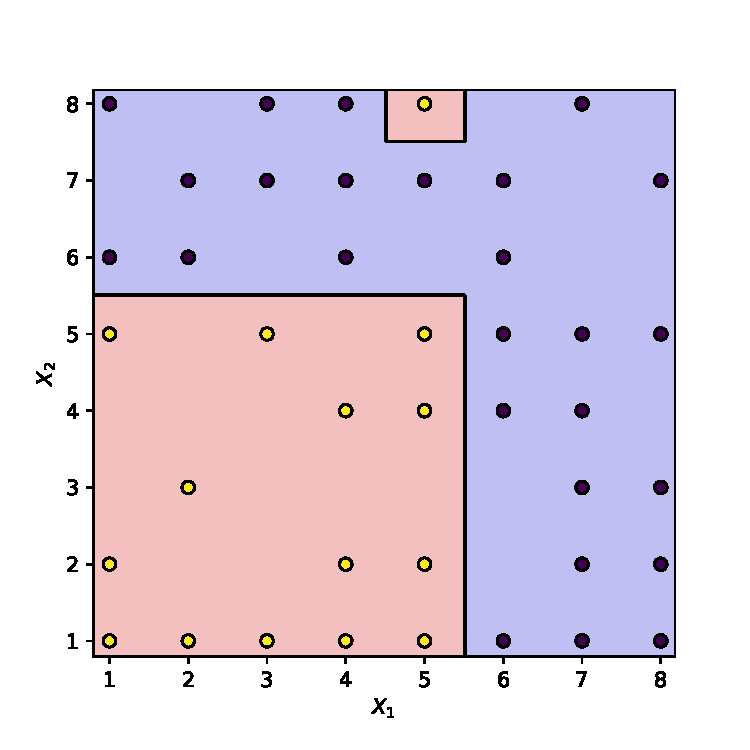
\includegraphics[width = 0.9\textwidth]{../assets/ensemble/figures/decision-boundary-4}}
      Tree Depth = 4

    \end{column}

  \end{columns}
\end{frame}

\begin{frame}{Bagging : Classification Example}
  Using majority voting to combine all predictions, we get the decision boundary below.\\
  \vspace{0.5cm}
  \centering
  \fitpic{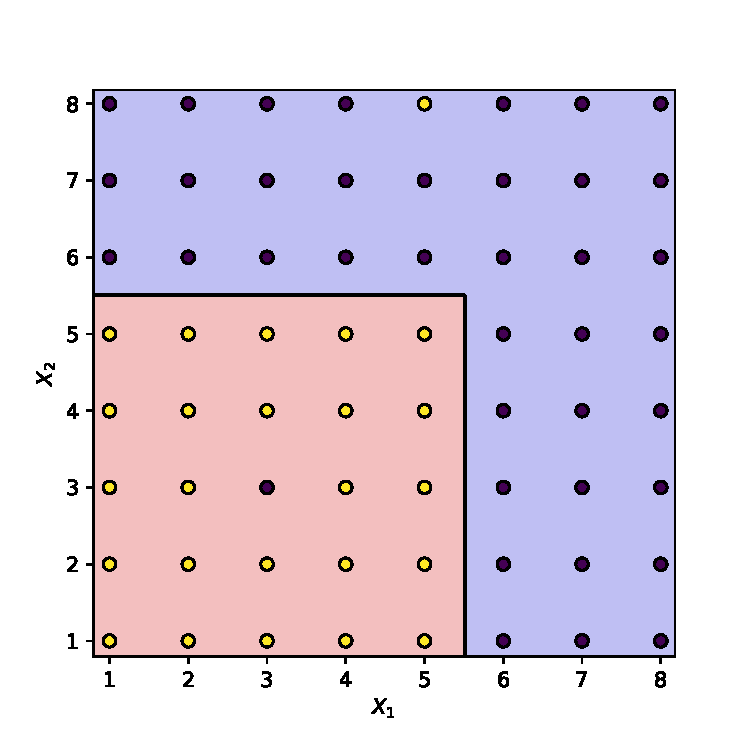
\includegraphics[width = 0.6\textwidth]{../assets/ensemble/figures/decision-boundary-ensemble}}
\end{frame}

\begin{frame}{Bagging}
  \textbf{Summary}
  \begin{itemize}
    \item We take ``strong'' learners and combine them to reduce variance.
    \item All learners are independent of each other.
  \end{itemize}
\end{frame}

\section{Boosting: Learning from Mistakes}

\begin{frame}{What is Boosting?}
\begin{definitionbox}{Boosting Philosophy}
\textbf{Goal:} Combine weak learners sequentially to create a strong ensemble
\end{definitionbox}

\begin{keypointsbox}
\textbf{Key Differences from Bagging:}
\begin{itemize}
\item \textbf{Sequential:} Models built one after another (not in parallel)
\item \textbf{Focus on Mistakes:} Each model learns from previous model's errors
\item \textbf{Reduce Bias:} Turn weak learners into strong ensemble
\end{itemize}
\end{keypointsbox}

\begin{examplebox}{The Boosting Intuition}
\textbf{``If at first you don't succeed, try harder on what you got wrong!''}
\end{examplebox}
\end{frame}

\begin{frame}{Boosting vs Bagging: Side-by-Side Comparison}
\begin{columns}
\begin{column}{0.48\textwidth}
\begin{alertbox}{Bagging}
\textbf{Strategy:} Parallel learning
\begin{itemize}
\item Models trained independently
\item Reduces variance
\item Works with ``strong'' learners
\item Bootstrap sampling
\item Simple majority voting
\end{itemize}
\end{alertbox}
\end{column}

\begin{column}{0.48\textwidth}
\begin{keypointsbox}{Boosting}
\textbf{Strategy:} Sequential learning
\begin{itemize}
\item Models learn from mistakes
\item Reduces bias
\item Works with ``weak'' learners
\item Weighted sampling
\item Weighted combination
\end{itemize}
\end{keypointsbox}
\end{column}
\end{columns}

\begin{definitionbox}{Weak Learner Definition}
\textbf{Weak Learner:} Any classifier that performs slightly better than random guessing (accuracy > 50% for binary classification)
\end{definitionbox}
\end{frame}

\begin{frame}{AdaBoost: Adaptive Boosting}
\begin{definitionbox}{AdaBoost Core Idea}
Each model adapts to previous model's mistakes
\end{definitionbox}

\begin{keypointsbox}
\textbf{Process:}
\begin{enumerate}
\item Train weak learner on weighted data
\item Increase weights of misclassified examples
\item Repeat: Focus on ``hard'' examples
\end{enumerate}
\end{keypointsbox}
\end{frame}

\begin{frame}{AdaBoost Step-by-Step: Problem Setup}
\begin{definitionbox}{AdaBoost Notation}
\begin{itemize}
\item $N$ training samples: $\{(x_1, y_1), (x_2, y_2), \ldots, (x_N, y_N)\}$
\item Sample weights: $w_i$ (importance of sample $i$ for training)
\item $M$ weak learners: $h_1, h_2, \ldots, h_M$
\item Learner weights: $\alpha_m$ (importance of learner $m$ in final ensemble)
\end{itemize}
\end{definitionbox}

  \vspace{0.3cm}
  \centering
  \fitpic{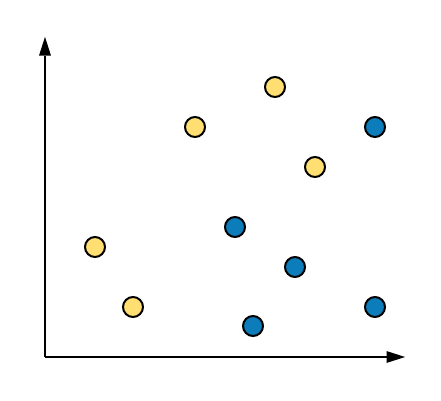
\includegraphics[width = 0.4\textwidth]{../assets/ensemble/diagrams/ada_data}}

\begin{keypointsbox}
\textbf{Goal:} Learn a strong classifier $H(x) = \text{sign}\left(\sum_{m=1}^M \alpha_m h_m(x)\right)$
\end{keypointsbox}
\end{frame}

\begin{frame}{AdaBoost Step 1: Initialize Sample Weights}
\begin{alertbox}{Step 1: Equal Importance for All Samples}
\textbf{Initialize:} $w_i^{(1)} = \frac{1}{N}$ for all $i = 1, 2, \ldots, N$
\end{alertbox}

\textbf{Why equal weights?}
\begin{itemize}
\item No prior knowledge about ``hard'' samples
\item Weights adapt as we learn from mistakes
\end{itemize}

  \vspace{0.3cm}
  \centering
  \fitpic{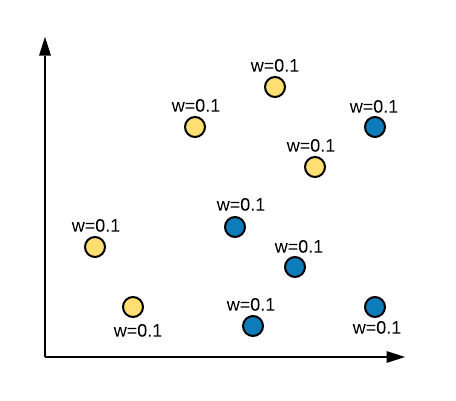
\includegraphics[width = 0.4\textwidth]{../assets/ensemble/diagrams/ada_data_init_weights}}
\end{frame}

\begin{frame}{AdaBoost Step 2: Train First Weak Learner}
\begin{alertbox}{Step 2a: Train Classifier on Weighted Data}
Train weak learner $h_1$ using current sample weights $w_i^{(1)}$
\end{alertbox}

\begin{keypointsbox}
\textbf{Key Insight:} Higher weight = more training focus
\begin{itemize}
\item Initially all weights equal → standard training
\end{itemize}
\end{keypointsbox}

  \vspace{0.3cm}
  \centering
  \fitpic{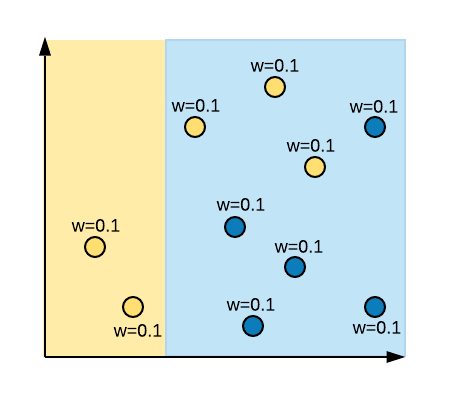
\includegraphics[width = 0.4\textwidth]{../assets/ensemble/diagrams/ada_iter1}}
\end{frame}

\begin{frame}{AdaBoost Step 2: Evaluate First Classifier}
\begin{alertbox}{Step 2b: Identify Mistakes}
First classifier $h_1$ makes some mistakes (shown in red crosses)
\end{alertbox}

\begin{keypointsbox}
\textbf{Important Observation:}
\begin{itemize}
\item Even weak learners make mistakes
\item These mistakes guide the next learning step
\item Key question: How much do we trust this classifier?
\end{itemize}
\end{keypointsbox}

  \vspace{0.3cm}
  \centering
  \fitpic{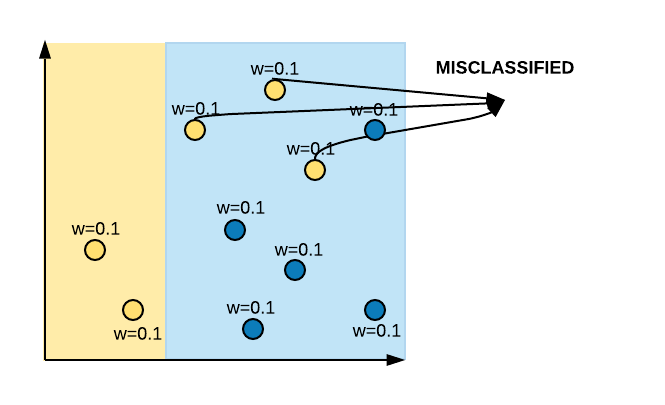
\includegraphics[width = 0.4\textwidth]{../assets/ensemble/diagrams/ada_iter1_misclassify}}

\begin{examplebox}{Teacher Analogy}
After first quiz, teacher sees which students got questions wrong
\end{examplebox}
\end{frame}

\begin{frame}{AdaBoost Step 3: Calculate Error}
\begin{definitionbox}{Weighted Error}
$$\text{err}_m = \frac{\text{weights of mistakes}}{\text{total weights}}$$
\end{definitionbox}

\begin{center}
\fitpic{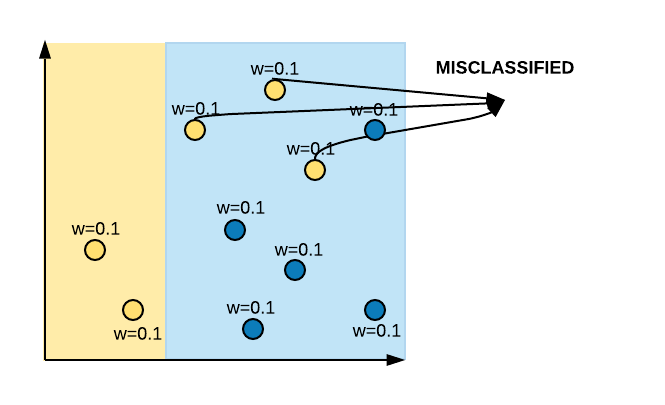
\includegraphics[width = 0.4\textwidth]{../assets/ensemble/diagrams/ada_iter1_misclassify}}
\end{center}

\begin{examplebox}{Example}
$err_1 = 0.3$ (30\% error → better than random)
\end{examplebox}
\end{frame}


\begin{frame}{AdaBoost Step 4: Calculate Classifier Weight}
\begin{definitionbox}{Classifier Weight Formula}
$$\alpha_m = \frac{1}{2}\ln\left(\frac{1 - \text{err}_m}{\text{err}_m}\right)$$
\textbf{Purpose:} Determine how much to trust this classifier in final ensemble
\end{definitionbox}

  \begin{columns}
    \begin{column}{0.5\textwidth}
      \centering
      \fitpic{\fitpic{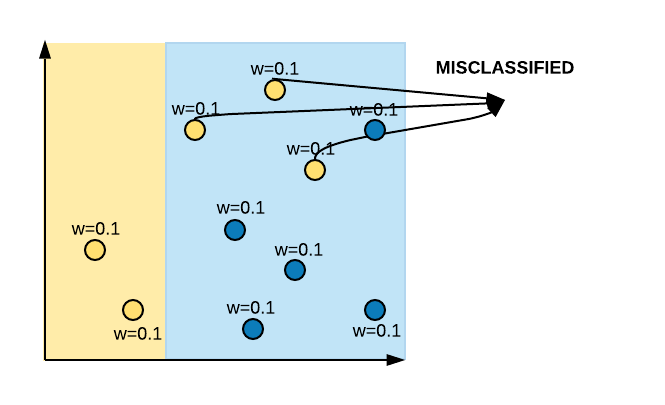
\includegraphics[width = \textwidth]{../assets/ensemble/diagrams/ada_iter1_misclassify}}}
    \end{column}
    \begin{column}{0.5\textwidth}
\begin{examplebox}{Example Calculation}
$err_1 = 0.3$

$\alpha_1 = \frac{1}{2}\ln\left(\frac{1-0.3}{0.3}\right) = \frac{1}{2}\ln(2.33) = 0.42$
\end{examplebox}

\begin{keypointsbox}
\textbf{Alpha Intuition:}
\begin{itemize}
\item Lower error → Higher $\alpha$
\item Higher $\alpha$ → More trust
\item $\alpha = 0$ when $err = 0.5$ (random)
\end{itemize}
\end{keypointsbox}
    \end{column}
  \end{columns}
\end{frame}

\begin{frame}{Understanding the Alpha Formula}
\begin{keypointsbox}
\textbf{What does } $\alpha = \frac{1}{2}\ln\left(\frac{1-err}{err}\right)$ \textbf{ really mean?}
\end{keypointsbox}

\begin{columns}
\begin{column}{0.5\textwidth}
\begin{definitionbox}{Perfect Classifier}
$err = 0 \Rightarrow \alpha = +\infty$

\textbf{Translation:} Infinite trust
\end{definitionbox}

\begin{examplebox}{Good Classifier}
$err = 0.1 \Rightarrow \alpha = 1.1$

\textbf{Translation:} High trust
\end{examplebox}
\end{column}

\begin{column}{0.5\textwidth}
\begin{alertbox}{Random Classifier}
$err = 0.5 \Rightarrow \alpha = 0$

\textbf{Translation:} No trust
\end{alertbox}

\begin{alertbox}{Worse than Random}
$err = 0.9 \Rightarrow \alpha = -1.1$

\textbf{Translation:} Negative trust (flip predictions!)
\end{alertbox}
\end{column}
\end{columns}

\begin{examplebox}{Key Insight}
\textbf{AdaBoost is mathematically elegant:} Even ``bad'' classifiers (worse than random) can be useful by flipping their predictions!
\end{examplebox}
\end{frame}

\begin{frame}{Boosting : AdaBoost }
  Consider we have a dataset of $N$ samples.\\
  Sample $i$ has weight $w_i$. There are $M$ classifiers in the ensemble.\\
  \begin{enumerate}
    \item Initialize weights of data samples: $w_i = \frac{1}{N}$
    \item For $m = 1, \ldots, M$:
          \begin{enumerate}
            \item Learn classifier using current weights $w_i$'s
            \item Compute the weighted error: $\text{err}_m = \frac{\sum_i w_i(\text{incorrect})}{\sum_i w_i}$
            \item Compute $\alpha_m = \frac{1}{2}\log_e\left(\frac{1 - \text{err}_m}{\text{err}_m}\right)$
            \item For samples which were predicted correctly: $w_i = w_i e^{-\alpha_m}$
            \item For samples which were predicted incorrectly: $w_i = w_i e^{\alpha_m}$
          \end{enumerate}
  \end{enumerate}
\end{frame}

\begin{frame}{Boosting : AdaBoost }
  \vspace{0.5cm}
  \centering
  \fitpic{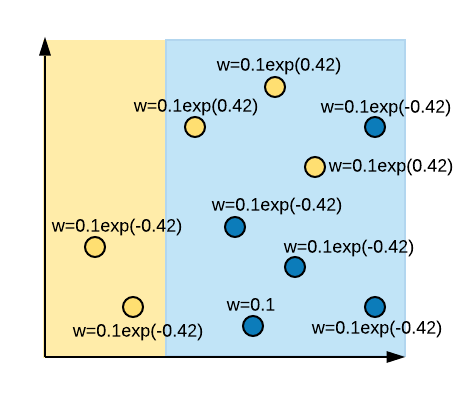
\includegraphics[width = 0.8\textwidth]{../assets/ensemble/diagrams/ada_iter1_new_weights_exp}}
\end{frame}

\begin{frame}{Boosting : AdaBoost }
  \vspace{0.5cm}
  \centering
  \fitpic{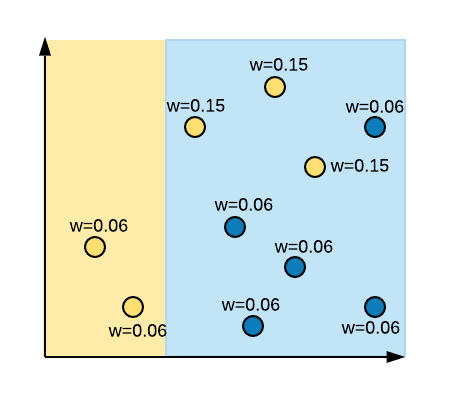
\includegraphics[width = 0.8\textwidth]{../assets/ensemble/diagrams/ada_iter1_new_weights}}
\end{frame}

\begin{frame}{Boosting : AdaBoost }
  Consider we have a dataset of $N$ samples.\\
  Sample $i$ has weight $w_i$. There are $M$ classifiers in the ensemble.\\
  \begin{enumerate}
    \item Initialize weights of data samples: $w_i = \frac{1}{N}$
    \item For $m = 1, \ldots, M$:
          \begin{enumerate}
            \item Learn classifier using current weights $w_i$'s
            \item Compute the weighted error: $\text{err}_m = \frac{\sum_i w_i(\text{incorrect})}{\sum_i w_i}$
            \item Compute $\alpha_m = \frac{1}{2}\log_e\left(\frac{1 - \text{err}_m}{\text{err}_m}\right)$
            \item For samples which were predicted correctly: $w_i = w_i e^{-\alpha_m}$
            \item For samples which were predicted incorrectly: $w_i = w_i e^{\alpha_m}$
            \item Normalize $w_i$'s to sum to 1.
          \end{enumerate}
  \end{enumerate}
\end{frame}

\begin{frame}{Boosting : AdaBoost }
  \vspace{0.5cm}
  \centering
  \fitpic{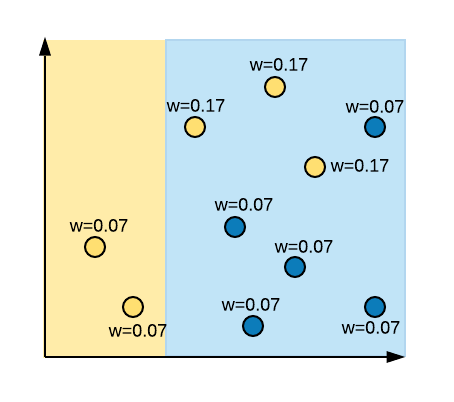
\includegraphics[width = 0.8\textwidth]{../assets/ensemble/diagrams/ada_iter1_new_weights_normalized}}
\end{frame}


\begin{frame}{Boosting : AdaBoost }
  Consider we have a dataset of $N$ samples.\\
  Sample $i$ has weight $w_i$. There are $M$ classifiers in the ensemble.\\
  \begin{enumerate}
    \item Initialize weights of data samples: $w_i = \frac{1}{N}$
    \item For $m = 1, \ldots, M$:
          \begin{enumerate}
            \item Learn classifier using current weights $w_i$'s
            \item Compute the weighted error: $\text{err}_m = \frac{\sum_i w_i(\text{incorrect})}{\sum_i w_i}$
            \item Compute $\alpha_m = \frac{1}{2}\log_e\left(\frac{1 - \text{err}_m}{\text{err}_m}\right)$
          \end{enumerate}
  \end{enumerate}
  \begin{columns}
    \begin{column}{0.5\textwidth}
      \centering
      \fitpic{\fitpic{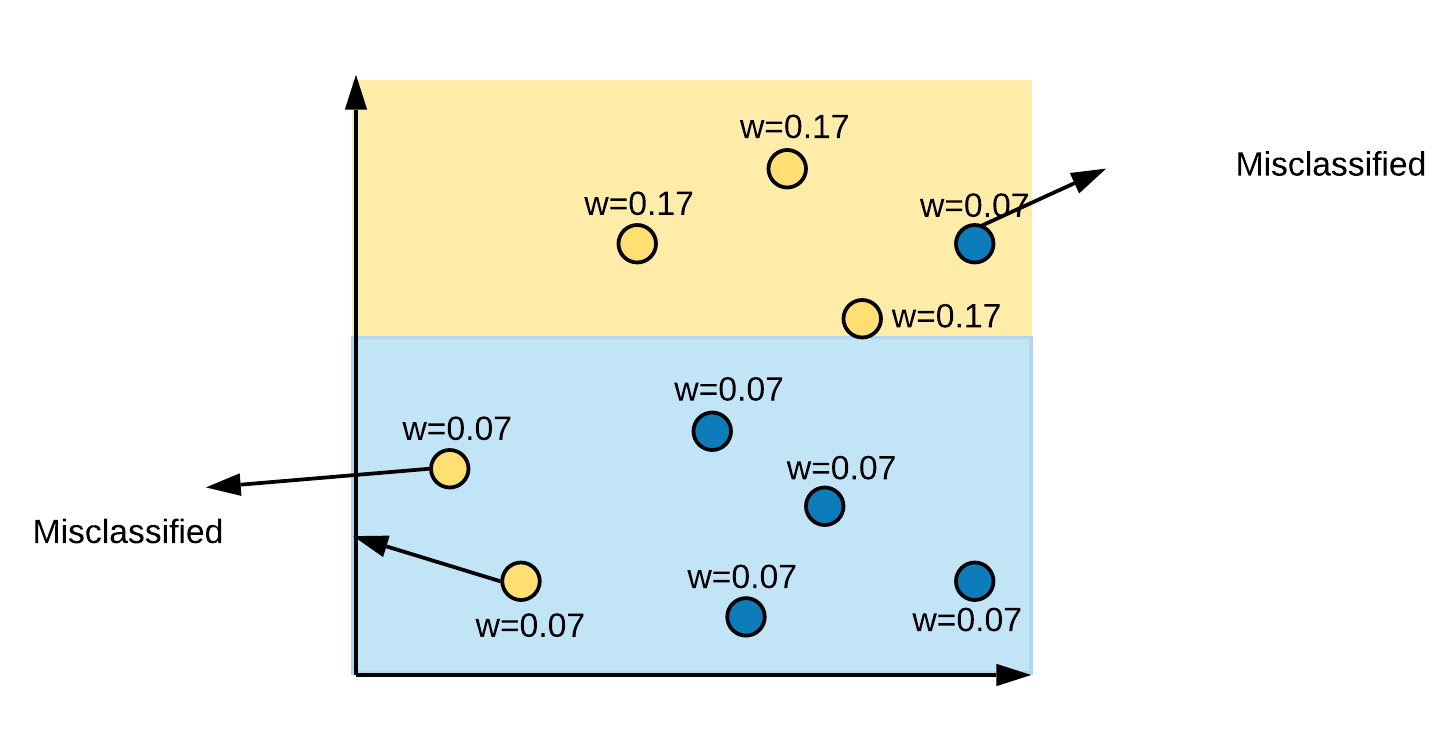
\includegraphics[width = \textwidth]{../assets/ensemble/diagrams/ada_iter2_misclassify}}}
    \end{column}
    \begin{column}{0.5\textwidth}
      $err_2 = \dfrac{0.21}{1}$\\
      $\alpha_2 = \dfrac{1}{2}log\left(\dfrac{1-0.21}{0.21}\right) = 0.66$
    \end{column}
  \end{columns}
\end{frame}

\begin{frame}{Boosting : AdaBoost }
  Consider we have a dataset of $N$ samples.\\
  Sample $i$ has weight $w_i$. There are $M$ classifiers in the ensemble.\\
  \begin{enumerate}
    \item Initialize weights of data samples: $w_i = \frac{1}{N}$
    \item For $m = 1, \ldots, M$:
          \begin{enumerate}
            \item Learn classifier using current weights $w_i$'s
            \item Compute the weighted error: $\text{err}_m = \frac{\sum_i w_i(\text{incorrect})}{\sum_i w_i}$
            \item Compute $\alpha_m = \frac{1}{2}\log_e\left(\frac{1 - \text{err}_m}{\text{err}_m}\right)$
            \item For samples which were predicted correctly: $w_i = w_i e^{-\alpha_m}$
            \item For samples which were predicted incorrectly: $w_i = w_i e^{\alpha_m}$
          \end{enumerate}
  \end{enumerate}
\end{frame}

\begin{frame}{Boosting : AdaBoost }
  \vspace{0.5cm}
  \centering
  \fitpic{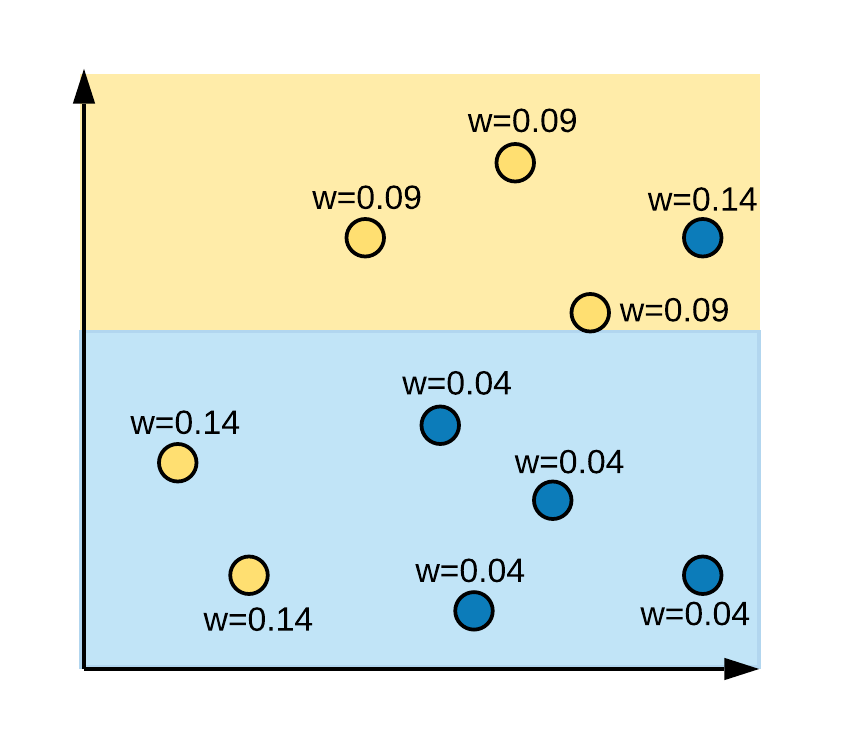
\includegraphics[width = 0.8\textwidth]{../assets/ensemble/diagrams/ada_iter2_new_weights}}
\end{frame}

\begin{frame}{Boosting : AdaBoost }
  Consider we have a dataset of $N$ samples.\\
  Sample $i$ has weight $w_i$. There are $M$ classifiers in the ensemble.\\
  \begin{enumerate}
    \item Initialize weights of data samples: $w_i = \frac{1}{N}$
    \item For $m = 1, \ldots, M$:
          \begin{enumerate}
            \item Learn classifier using current weights $w_i$'s
            \item Compute the weighted error: $\text{err}_m = \frac{\sum_i w_i(\text{incorrect})}{\sum_i w_i}$
            \item Compute $\alpha_m = \frac{1}{2}\log_e\left(\frac{1 - \text{err}_m}{\text{err}_m}\right)$
            \item For samples which were predicted correctly: $w_i = w_i e^{-\alpha_m}$
            \item For samples which were predicted incorrectly: $w_i = w_i e^{\alpha_m}$
            \item Normalize $w_i$'s to sum to 1.
          \end{enumerate}
  \end{enumerate}
\end{frame}

\begin{frame}{Boosting : AdaBoost }
  \vspace{0.5cm}
  \centering
  \fitpic{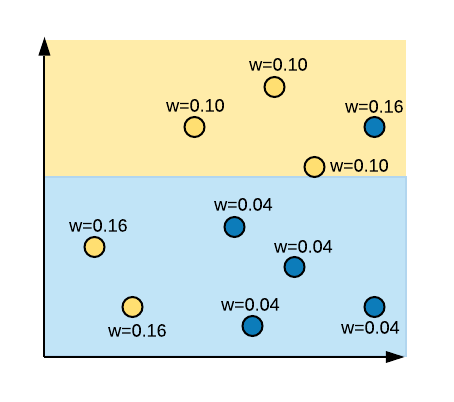
\includegraphics[width = 0.8\textwidth]{../assets/ensemble/diagrams/ada_iter2_new_weights_normalized}}
\end{frame}


\begin{frame}{Boosting : AdaBoost }
  Consider we have a dataset of $N$ samples.\\
  Sample $i$ has weight $w_i$. There are $M$ classifiers in the ensemble.\\
  \begin{enumerate}
    \item Initialize weights of data samples: $w_i = \frac{1}{N}$
    \item For $m = 1, \ldots, M$:
          \begin{enumerate}
            \item Learn classifier using current weights $w_i$'s
            \item Compute the weighted error: $\text{err}_m = \frac{\sum_i w_i(\text{incorrect})}{\sum_i w_i}$
            \item Compute $\alpha_m = \frac{1}{2}\log_e\left(\frac{1 - \text{err}_m}{\text{err}_m}\right)$
          \end{enumerate}
  \end{enumerate}
  \begin{columns}
    \begin{column}{0.5\textwidth}
      \centering
      \fitpic{\fitpic{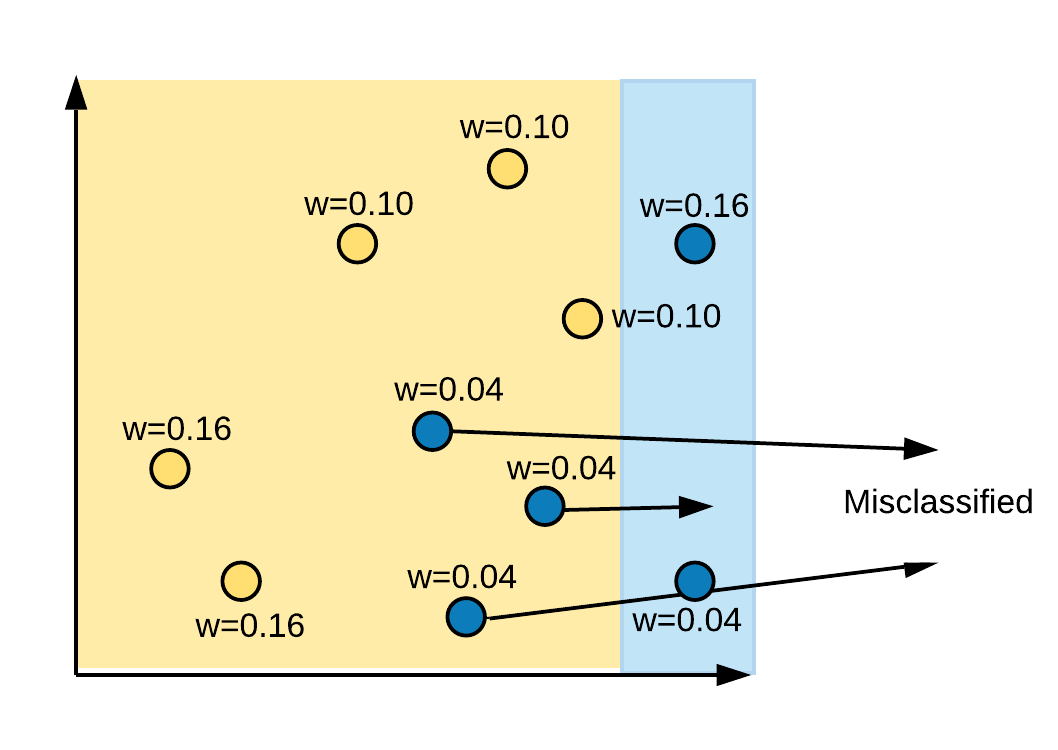
\includegraphics[width = \textwidth]{../assets/ensemble/diagrams/ada_iter3_misclassify}}}
    \end{column}
    \begin{column}{0.5\textwidth}
      $err_3 = \dfrac{0.12}{1}$\\
      $\alpha_3 = \dfrac{1}{2}log\left(\dfrac{1-0.12}{0.12}\right) = 0.99$
    \end{column}
  \end{columns}
\end{frame}

\begin{frame}{Boosting: Adaboost}
  Intuitively, after each iteration, importance of wrongly classified samples is increased by increasing their weights and importance of correctly classified     samples is decreased by decreasing their weights.
\end{frame}

\begin{frame}{Boosting: Adaboost}
  \textbf{Testing}\\
  \begin{itemize}
	\item For each sample $x$, compute the prediction of each classifier $h_m(x)$.
	\item Final prediction is the sign of the sum of weighted predictions, given as:
	\item SIGN($\alpha_1 h_1(x)$ +  $\alpha_2 h_2(x)$ + $\dots$ +  $\alpha_M h_M(x)$)
  \end{itemize}

\end{frame}

\begin{frame}{Boosting: Adaboost}
  \textbf{Example}
	\begin{columns}
		\pause 			\begin{column}{0.33\textwidth}
				\centering
				\begin{figure}
					\fitpic{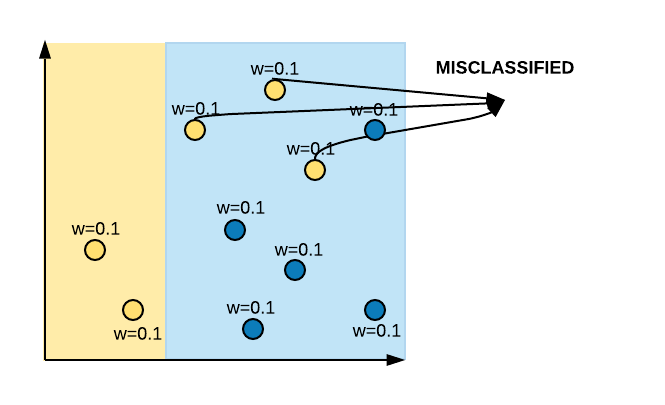
\includegraphics[width = \textwidth]{../assets/ensemble/diagrams/ada_iter1_misclassify}}
									\vspace{-20pt}
					\caption{$\alpha_1=0.42$}
				\end{figure}
				
			\end{column}
			
			
			\pause \begin{column}{0.4\textwidth}
				\centering
				\begin{figure}
					\fitpic{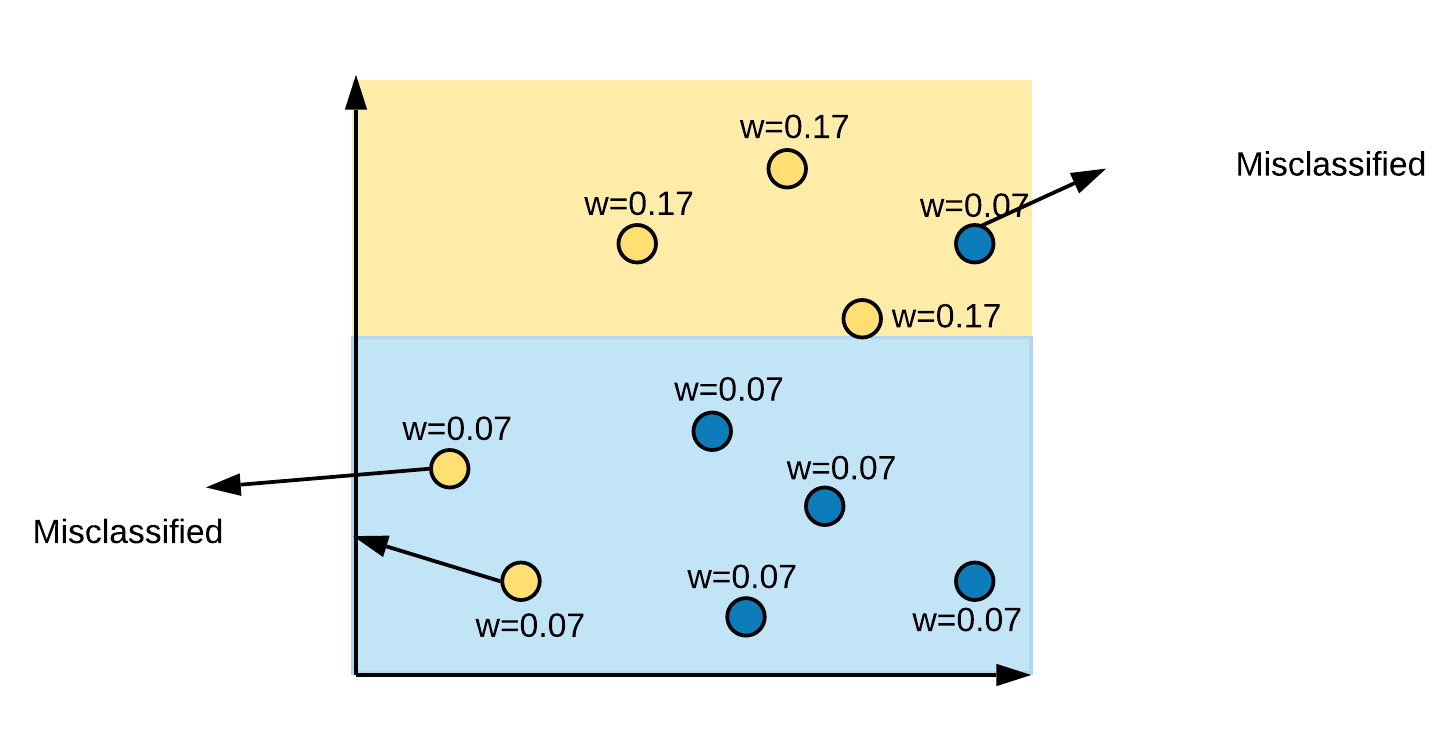
\includegraphics[width = \textwidth]{../assets/ensemble/diagrams/ada_iter2_misclassify}}
					\vspace{-20pt}
					\caption{$\alpha_2=0.66$}
				\end{figure}
	
			\pause \end{column}
					\begin{column}{0.3\textwidth}
				\centering
				\begin{figure}
					\fitpic{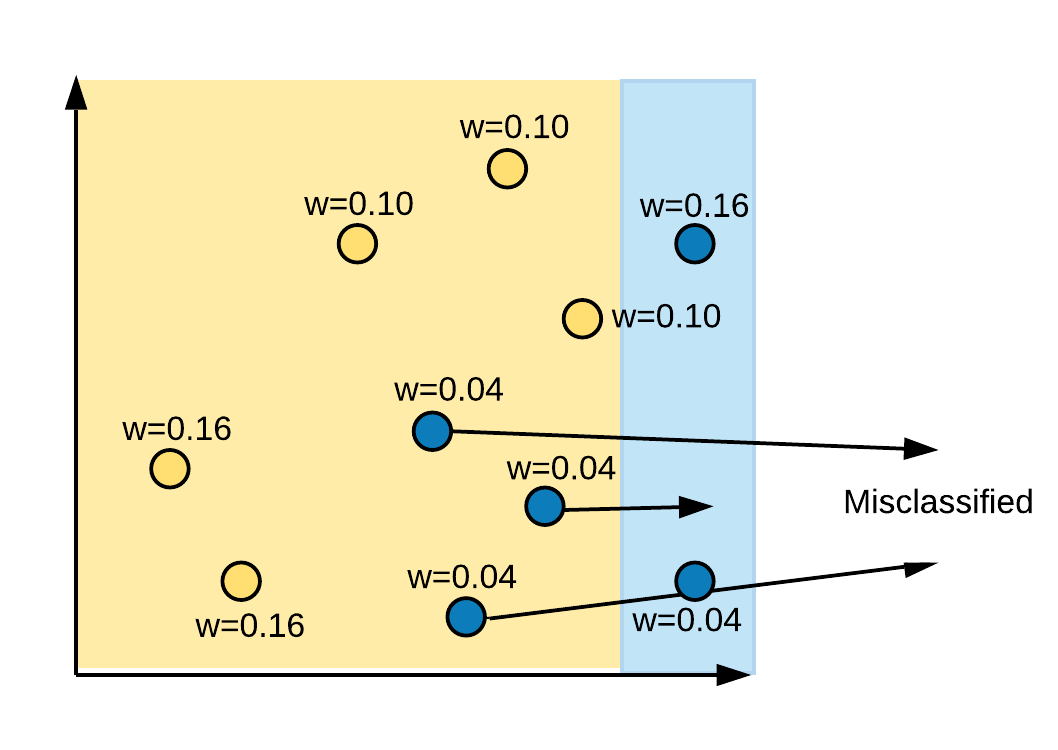
\includegraphics[width = \textwidth]{../assets/ensemble/diagrams/ada_iter3_misclassify}}
									\vspace{-20pt}
					\caption{$\alpha_3=0.99$}
				\end{figure}
				
			\end{column}
		\end{columns}
	
		\begin{columns}
			\pause \begin{column}{0.5\textwidth}
				\begin{figure}
				\fitpic{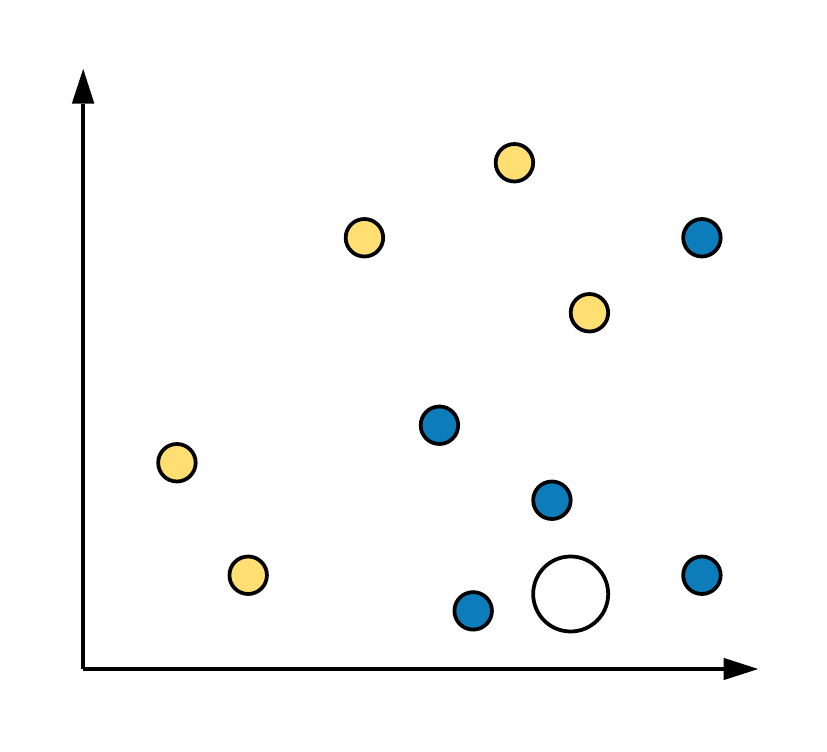
\includegraphics[scale=0.1]{../assets/ensemble/diagrams/testing}}
				\end{figure}
			\end{column}
		
		\begin{column}{0.5\textwidth}
			\pause Let us say, yellow class is +1 and blue class is -1
			
			\pause Prediction = SIGN(0.42*-1 + 0.66*-1 + 0.99*+1) = Negative = blue
		\end{column}
		\end{columns}
	
\end{frame}

% \begin{frame}

%     \pause \begin{column}{0.4\textwidth}
%       \centering
%       \begin{figure}
%         \fitpic{\fitpic{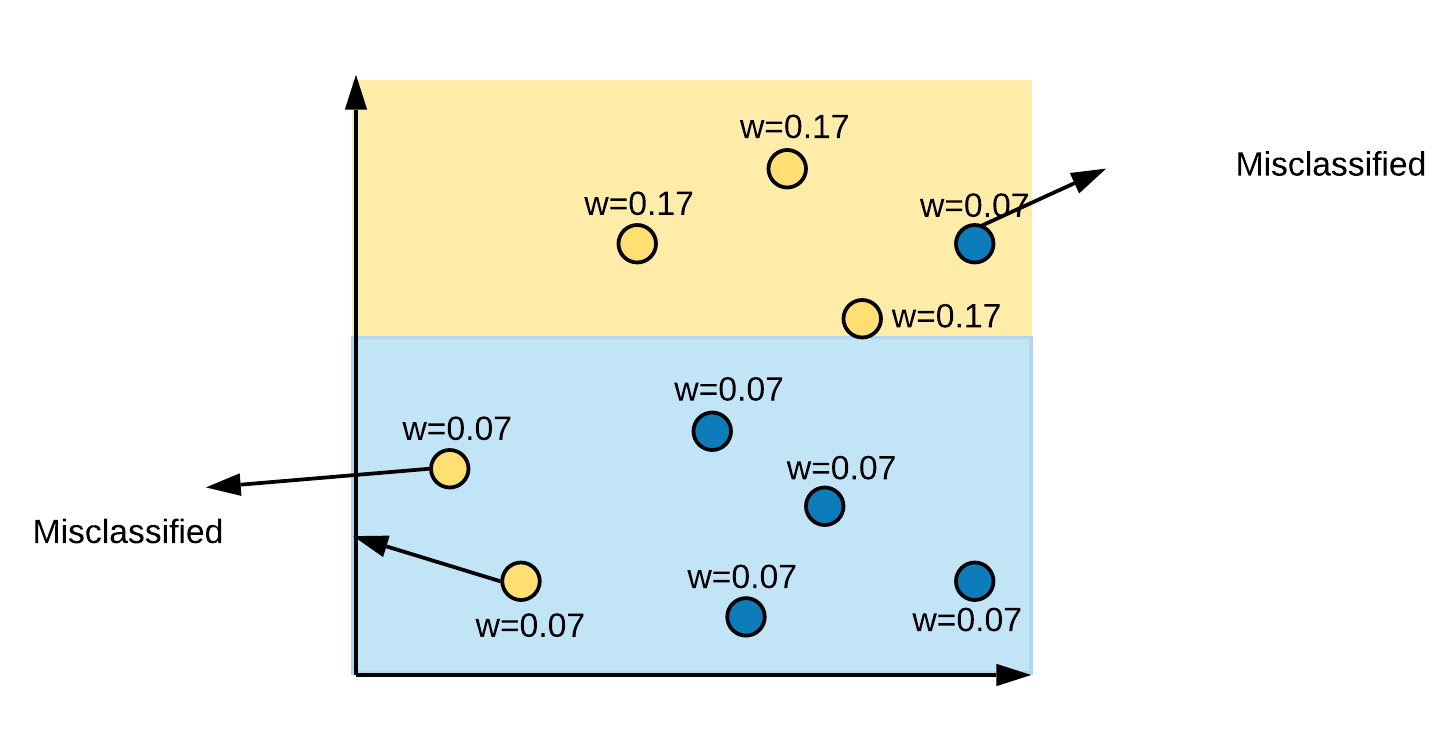
\includegraphics[width = \textwidth]{../assets/ensemble/diagrams/ada_iter2_misclassify}}}
%         \vspace{-20pt}
%         \caption{$\alpha_2=0.66$}
%       \end{figure}
% 	\end{column}
% \end{columns}

% \end{frame}
		
% 	\begin{frame}
%       \pause \end{column}
%     \begin{column}{0.3\textwidth}
%       \centering
%       \begin{figure}
%         \fitpic{\fitpic{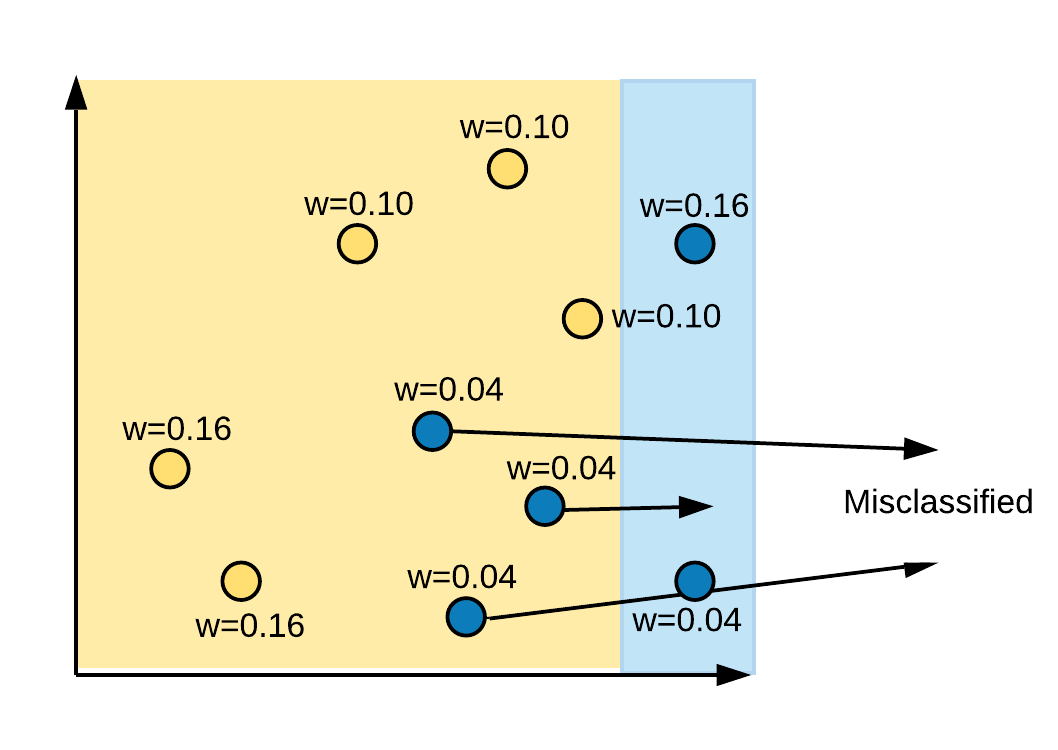
\includegraphics[width = \textwidth]{../assets/ensemble/diagrams/ada_iter3_misclassify}}}
%         \vspace{-20pt}
%         \caption{$\alpha_3=0.99$}
%       \end{figure}

%     \end{column}
%   \end{columns}

%   \begin{columns}
%     \pause \begin{column}{0.5\textwidth}
%       \begin{figure}
%         \fitpic{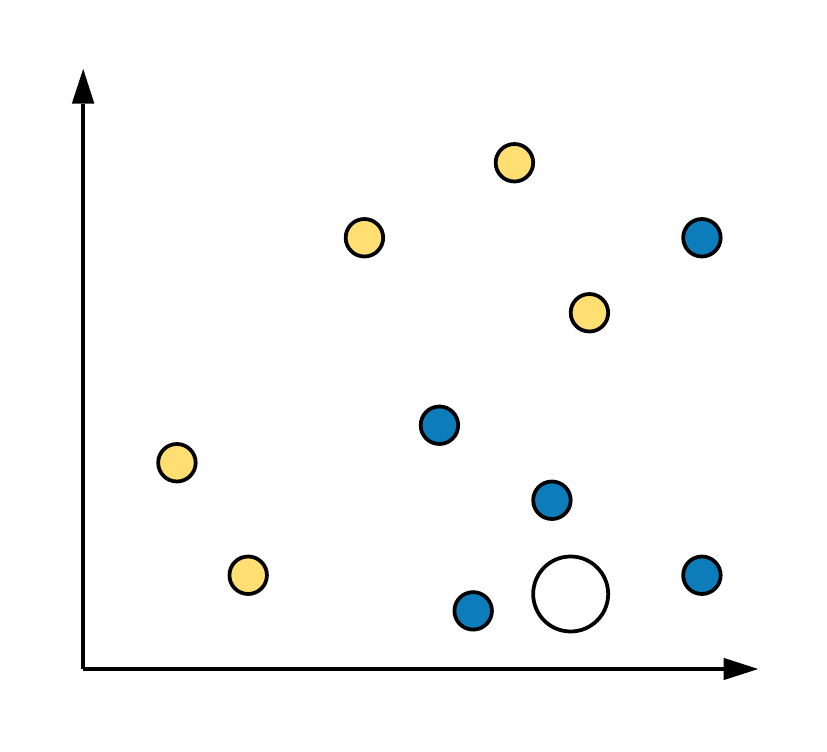
\includegraphics[scale=0.1]{../assets/ensemble/diagrams/testing}}
%       \end{figure}
%     \end{column}

%     \begin{column}{0.5\textwidth}
%       \pause Let us say, yellow class is +1 and blue class is -1

%       \pause Prediction = SIGN(0.42*-1 + 0.66*-1 + 0.99*+1) = Negative = blue
%     \end{column}
%   \end{columns}

% \end{frame}


\begin{frame}{Intuition behind weight update formula}
  \begin{columns}
    \pause \begin{column}{0.5\textwidth}

      \begin{figure}[htp]
        \centering
        \begin{notebookbox}{https://nipunbatra.github.io/ml-teaching/notebooks/boosting-explanation.html}
          % 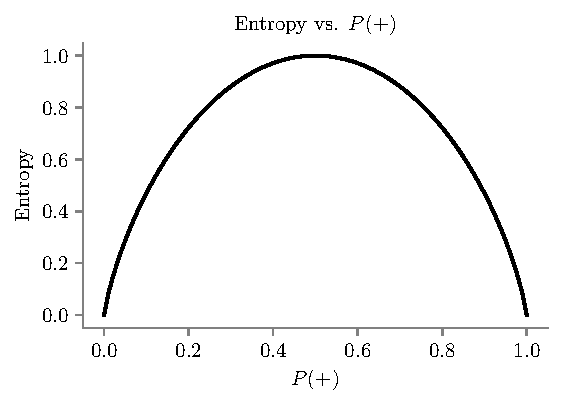
\includegraphics[scale=0.8]{../figures/decision-trees/entropy.pdf}
          \fitpic{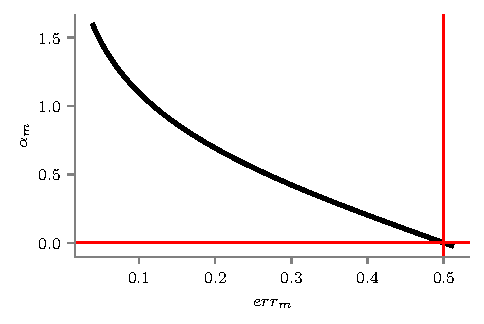
\includegraphics[scale=0.55]{../assets/ensemble/figures/alpha-boosting.pdf}}
        \end{notebookbox}
      \end{figure}
    \end{column}
    \pause \begin{column}{0.5\textwidth}
      \begin{figure}[htp]
        \centering
        \begin{notebookbox}{https://nipunbatra.github.io/ml-teaching/notebooks/boosting-explanation.html}
          \fitpic{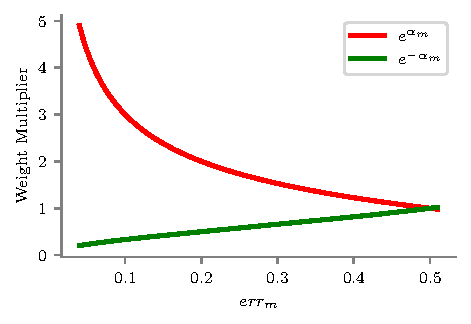
\includegraphics[scale=0.55]{../assets/ensemble/figures/alpha-boosting-weight.pdf}}
        \end{notebookbox}
      \end{figure}
    \end{column}
  \end{columns}


\end{frame}

\begin{frame}{ADABoost for regresion}
  From Paper: Improving Regressors using Boosting Techniques

  \fitpic{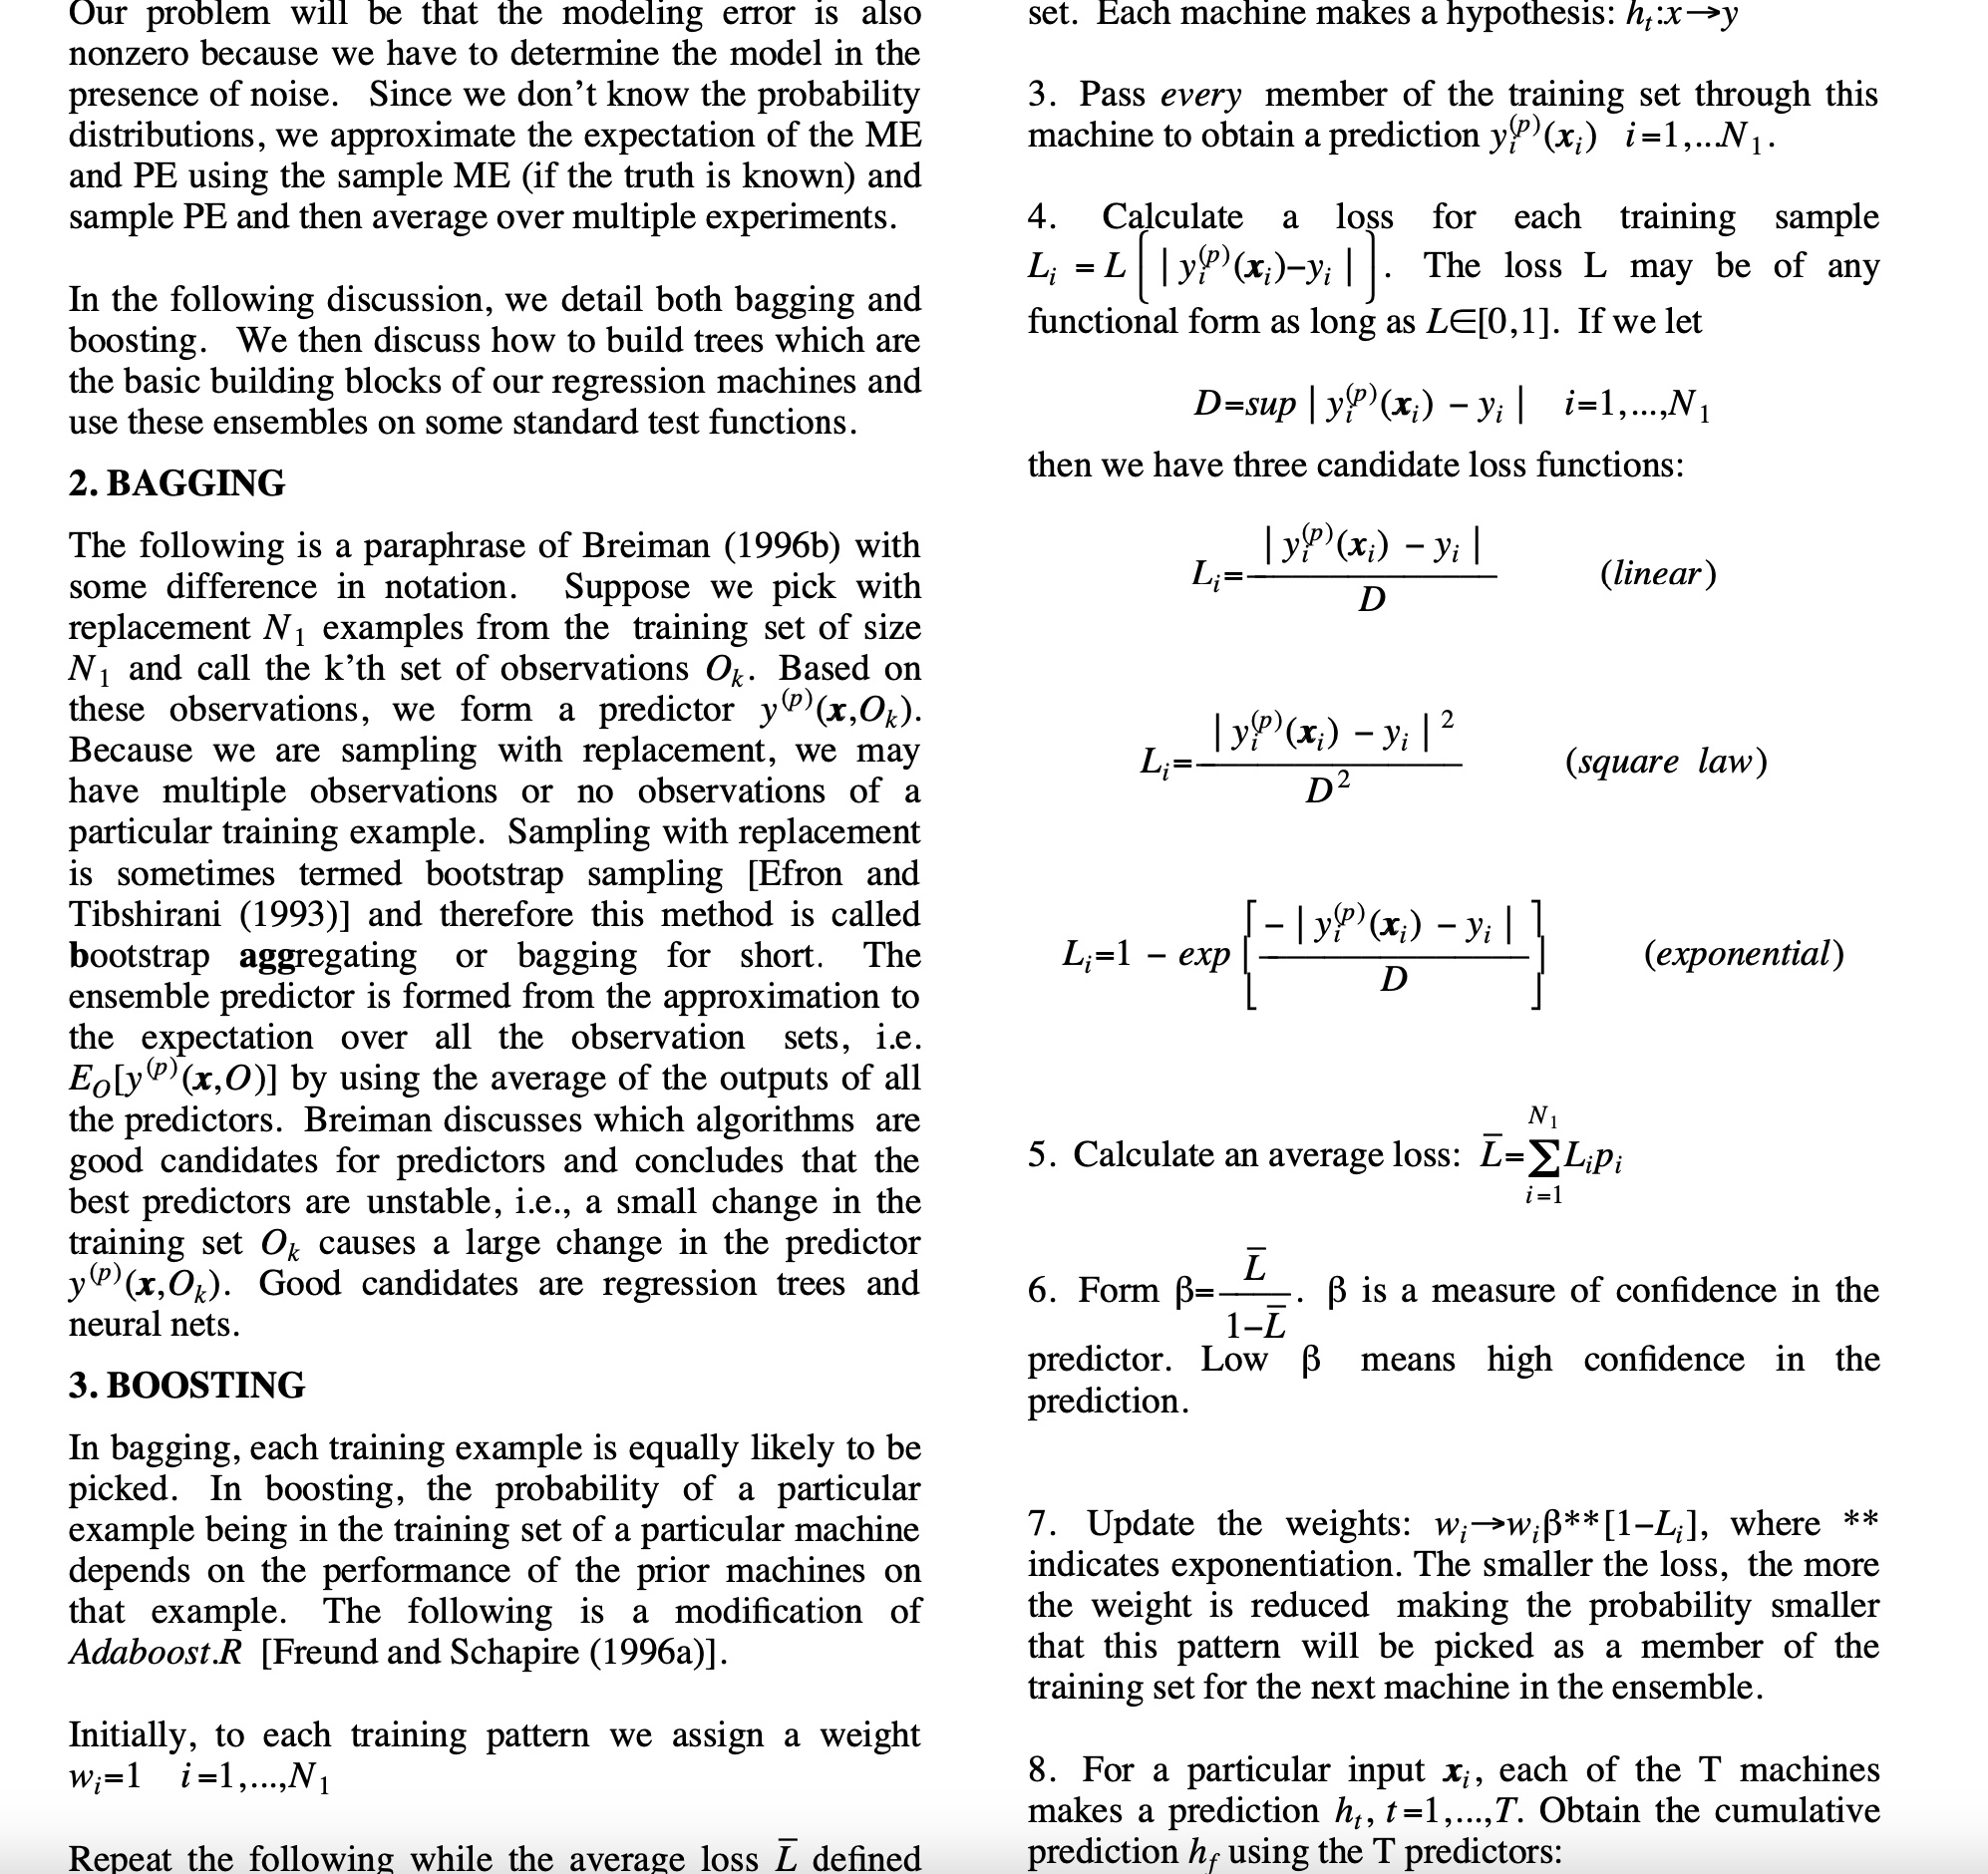
\includegraphics[scale=0.1]{../assets/ensemble/diagrams/adaboost-regression.jpg}}
  
\end{frame}

\section{Random Forest: Double Randomness}

\begin{frame}{What is Random Forest?}
\begin{definitionbox}{Random Forest = Bagging + Feature Randomness}
\textbf{Core Idea:} Combine many decision trees trained on random subsets of data AND random subsets of features
\end{definitionbox}

\begin{keypointsbox}
\textbf{Two Sources of Randomness:}
\begin{itemize}
\item \textbf{Bootstrap Sampling:} Each tree sees different training samples (like bagging)
\item \textbf{Feature Subsampling:} Each split considers only random subset of features
\end{itemize}
\end{keypointsbox}

\begin{examplebox}{Why Double Randomness?}
\textbf{Goal:} Create diverse trees that make different mistakes
\begin{itemize}
\item Data randomness → Different perspectives on the problem
\item Feature randomness → Different decision criteria
\item Result: Highly decorrelated predictions!
\end{itemize}
\end{examplebox}
\end{frame}

\begin{frame}{Random Forest Algorithm: Step by Step}
\begin{definitionbox}{Random Forest Hyperparameters}
\begin{itemize}
\item $B$ = Number of trees in the forest
\item $m$ = Number of features considered at each split (typically $\sqrt{M}$ or $\log_2(M)$)
\item $\text{max\_depth}$ = Maximum depth of each tree
\end{itemize}
\end{definitionbox}

\begin{alertbox}{Random Forest Training Algorithm}
\textbf{For } $b = 1, 2, \ldots, B$:
\begin{enumerate}
\item \textbf{Bootstrap:} Sample $n$ training examples with replacement
\item \textbf{Train Tree:} Build tree with feature randomness:
\begin{itemize}
\item At each split: randomly select $m$ out of $M$ features
\item Choose best split among these $m$ features only
\end{itemize}
\end{enumerate}
\end{alertbox}

\begin{keypointsbox}
\textbf{Key Insight:} Each tree is ``strong'' individually but they make different mistakes due to randomness!
\end{keypointsbox}
\end{frame}

\begin{frame}{Random Forest: Feature Selection at Each Split}
\begin{examplebox}{Iris Example}
\textbf{4 features available} $\Rightarrow$ $m = \sqrt{4} = 2$ features per split
\end{examplebox}

\begin{columns}
\begin{column}{0.48\textwidth}
\begin{definitionbox}{Tree 1 - Split 1}
\textbf{Random subset:} \{Sepal Length, Petal Width\}

\textbf{Best split:} Petal Width $< 0.8$
\end{definitionbox}
\end{column}

\begin{column}{0.48\textwidth}
\begin{definitionbox}{Tree 2 - Split 1}
\textbf{Random subset:} \{Sepal Width, Petal Length\}

\textbf{Best split:} Petal Length $< 2.5$
\end{definitionbox}
\end{column}
\end{columns}

\begin{keypointsbox}
\textbf{Result:} Different trees focus on different feature combinations → Diverse predictions
\end{keypointsbox}
\end{frame}

\begin{frame}{Random Forest Example: Iris Dataset}
\begin{examplebox}{The Iris Classification Problem}
\textbf{Task:} Classify iris flowers into 3 species based on 4 measurements
\end{examplebox}

  \vspace{0.3cm}
  \centering
  \fitpic{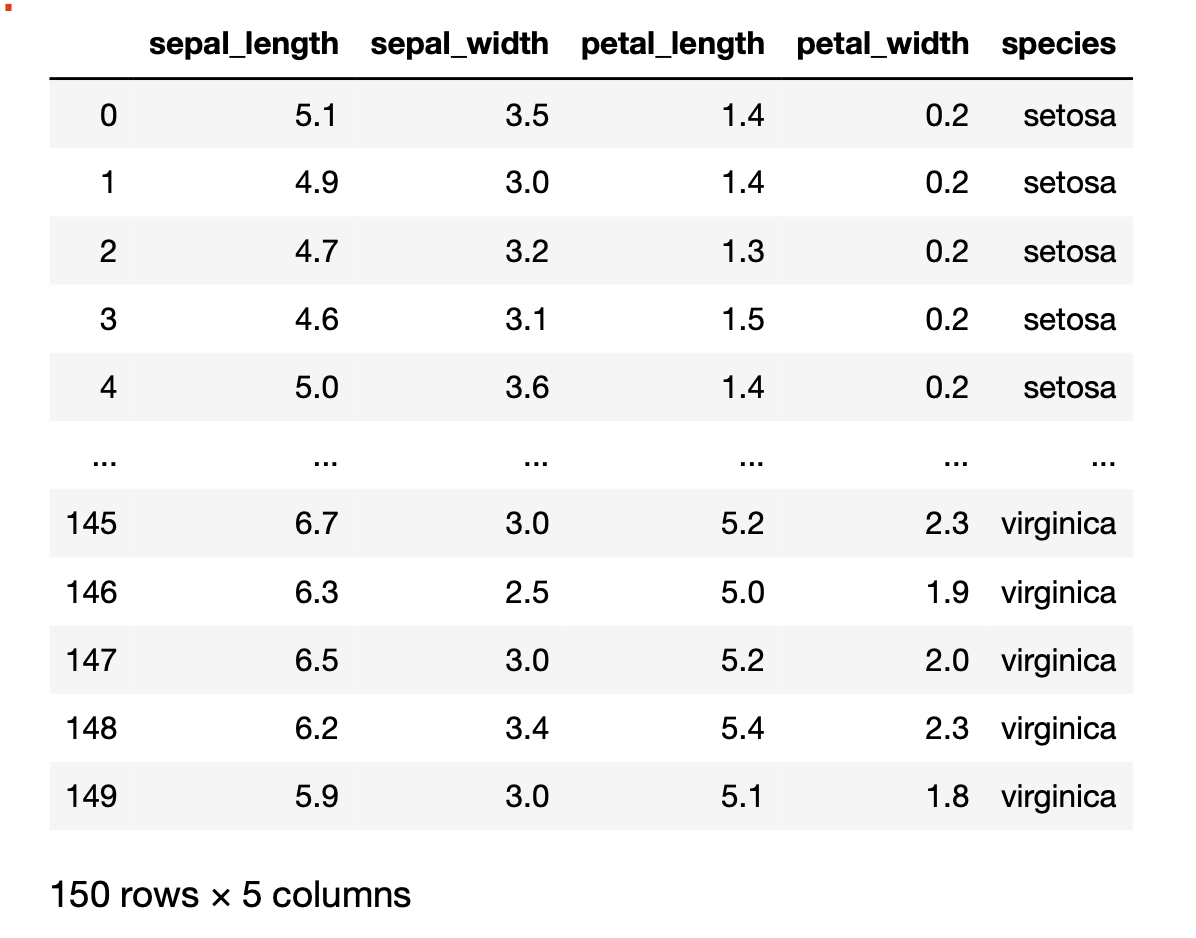
\includegraphics[scale=0.5]{../assets/ensemble/diagrams/dataset-iris.png}}

\begin{keypointsbox}
\textbf{Random Forest Setup:}
\begin{itemize}
\item 4 features available → Consider $m = 2$ features per split
\item Bootstrap samples for each tree
\item Combine predictions via majority voting
\end{itemize}
\end{keypointsbox}
\end{frame}


% \begin{frame}{Random Forest}
% There are 3 parameters while training a random forest ``$number$ $of$ $trees$'', ``$number$ $of$ $features'' (m)$, ``$maximum$ $depth$''.\\
% \vspace{1cm}
% \underline{Training Algorithm}\\
% \begin{itemize}
%   \item for $depth$ in $[1, \dots,$ $maximum$ $depth$ $]$
%     \begin{itemize}
%       \item for $tree$ in $[1, \dots,$ $number$ $of$ $trees$ $]$
%       \begin{itemize}
%         \item For each split, select ``$m$'' features from total available $M$ features and train a decision tree on selected features
%         
%       \end{itemize}
%     \end{itemize}
% \end{itemize}
% \end{frame}



\newcounter{tree}
\forloop{tree}{0}{\value{tree} < 10}{
  \begin{frame}{Decision Tree \# \thetree}
    \begin{figure}
      % \includegraphics[scale=0.25]{../assets/ensemble/figures/feature-imp-\thetree.pdf}
      \centering
      \begin{notebookbox}{https://nipunbatra.github.io/ml-teaching/notebooks/ensemble-feature-importance.html}
        \fitpic{\includegraphics[scale=0.25]{../assets/ensemble/figures/feature-imp-\thetree.pdf}}
        
      \end{notebookbox}
    \end{figure}
  \end{frame}
}


\begin{frame}{Feature Importance\footnotemark}
  \begin{figure}
    \fitpic{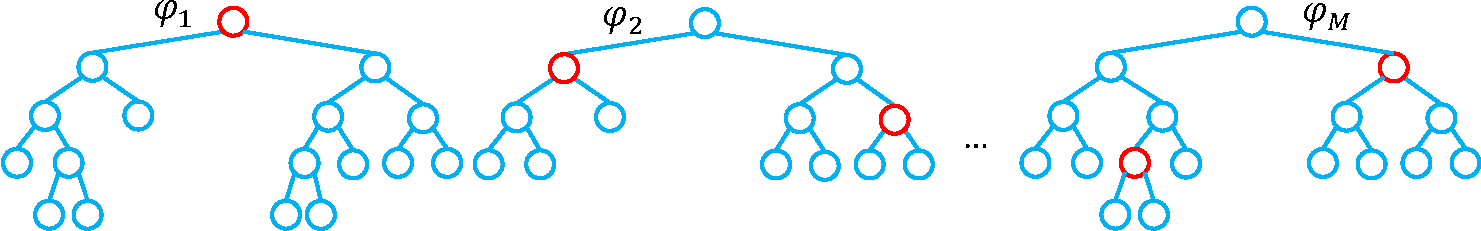
\includegraphics[scale=0.4]{../assets/ensemble/diagrams/mdi.pdf}}
  \end{figure}
  Importance of variable $X_j$ for an ensemble of $M$ trees $\varphi_{m}$ is:
  \begin{equation*}
    \text{Imp}(X_j) = \frac{1}{M} \sum_{m=1}^M \sum_{t \in \varphi_{m}} 1(j_t = j) \Big[ p(t) \Delta i(t) \Big],
  \end{equation*}
  where $j_t$ denotes the variable used at node $t$, $p(t)=N_t/N$ and $\Delta i(t)$ is the impurity reduction at node $t$:
  \begin{equation*}
    \Delta i(t) = i(t) - \frac{N_{t_L}}{N_t} i(t_L) - \frac{N_{t_r}}{N_t} i(t_R)
  \end{equation*}
  \footnotetext[1]{Slide Courtesy Gilles Louppe}

\end{frame}


\begin{frame}{Computed Feature Importance}
  \begin{figure}[htp]
    \centering
    \begin{notebookbox}{https://nipunbatra.github.io/ml-teaching/notebooks/ensemble-feature-importance.html}
      \fitpic{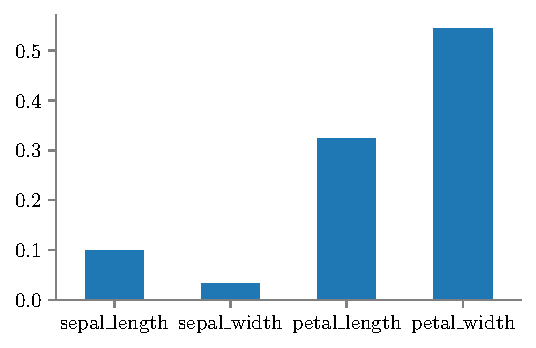
\includegraphics[scale=0.8]{../assets/ensemble/figures/feature-imp-forest.pdf}}
    \end{notebookbox}
\end{figure}
  % 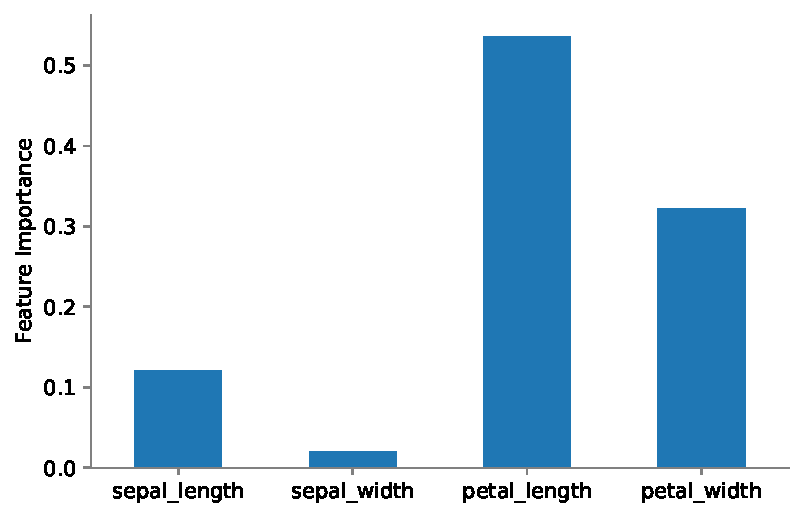
\includegraphics[scale=0.6]{feature-importance.pdf}
\end{frame}

\end{document}
